
\chapter{Scheduling Unsynchronized Periodic Datagrams without Buffer}
\label{chap:PAZL}
\minitoc


This chapter corresponds to two articles: Section $3$ of~\cite{DBLP:conf/ict/BarthGLMS18} and all of~\cite{DBLP:journals/corr/abs-2002-07606}.


 In this chapter, we propose algorithm to solve the problem \pazl on \emph{star routed networks}, a problem denoted by \textsc{PMA}\xspace for \textbf{P}eriodic \textbf{M}essage \textbf{A}ssignment in~\cite{DBLP:journals/corr/abs-2002-07606}.
 In this context, once a datagram has been emitted, no buffering is allowed in the network for contention. Remark that, if some buffering is necessary 
 for dealing with some technical difficulty, but its duration is deterministic, it can be encoded into the length of the links.
 The bufferless assignment we design may allow to design completely bufferless networks, using full optical networks or new generation of networks mentionned in Chapter~\ref{chap:TSN}, which provide transparent transmission of data without latency inducing opto-electronic conversion or forwarding computations. 

 In the problem \pma (and also in the problem \pall studied in Chapter~\ref{chap:PALL}), the datagram emissions are not synchronized. This means the sources don't send the datagram at the same time in the period. This is why we can choose the offset on the period without adding latency to the datagram. Such a problem does not perfectly match with C-RAN in actual 5G, but can be used in many other applications in which the sources do not need to be synchronized (industry 4.0, monitoring, sensor network, multicore over a bus, two processors scheduling, \dots).  Moreover, we hope that future evolutions of the 5G standard will allow to use unsynchronized antennas.

 Since \pma is a more constrained problem than \pall, we simplify the notations. No buffering is allowed, hence the notion of deadline on each route is not relevant anymore because all datagrams have the smallest possible process time, if there is a solution. Thus, an instance of \pma can be given, for each route $i$, by the length of the arc $(c_1,c_2)$ on $r_i$, that is $\omega(r_i,c_1)$, denoted in this chapter by $\notationdelay_i$ and called \nomdelay. A datagram is emitted an infinite number of times periodically, hence it is enough to consider any interval of $P$ units of time to completely represent the state of our system by giving the times, in this interval, at which each datagram goes through the two contention points. We call the representation of an interval of $P$ units of time in the first contention point the \textbf{first period} and the \textbf{second period} for the second contention point. 

 Recall that an \textbf{offset} of a datagram is a choice of time at which it arrives
 at the first contention point (i.e. in the first period). Let us consider a datagram $i$
 of offset $o_i$, it uses the interval of time $[i]_1 = \{ (o_i + t) \mod P \mid 0 \leq t < \tau \}$ in the first period and $[i]_2 = \{ (d_i + o_i + t) \mod P \mid 0 \leq t < \tau \}$ in the second period. Two datagrams $i$ and $j$ \textbf{collide} if either $[i]_1 \cap [j]_1 \neq \emptyset $ or $[i]_2 \cap [j]_2 \neq \emptyset $. If $t \in [i]_1$ (resp. $t \in [i]_2$), we say that datagram $i$ uses time $t$ in the first period (resp. in the second period). An \textbf{assignment} is a function from the datagrams to their offsets, such that there is no collision.


The complexity of \pma on star routed networks is yet unknown. We prove in this chapter that, when parameterized by
$n$ the number of datagrams, the problem is \FPT. On a slight generalization of the star routed network, with more contention points, but each datagram only going through two of them, \pazl is \NP-hard, see Theorem~\ref{th:hardness_contention_depth}. When the shared link is not full-duplex, that is, there is a single contention point and each datagram goes through it twice, we can encode the same non periodic problem, which is \NP-hard~\cite{orman1997complexity}. Hence, we conjecture that \pma is \NP-hard.

To overcome the supposed hardness of \pma, we study it when the load of the system is small enough, which is defined here as
the number of units of time used in a period by all datagrams divided by the period that is $n\tau /P$. There cannot be an assignment when the load is larger than one; \textbf{we prove in this chapter that, for moderate loads, there is \emph{always} an assignment and that it can be found by a polynomial time algorithm}. When an algorithm finds an assignment to the problem \pma, for any input in some set, we say it solves \pma \textbf{positively} on the set of inputs. This kind of result is very helpful when solving the following optimization version of \pma: given a set of datagrams, find the largest subset which admits an assignment. A weighted version, where the datagrams have different size can also be considered. An optimal solution to the optimization problem is a set of datagrams corresponding to a load of at most $1$. Assume we have an algorithm that always finds an assignment for an instance of load $\lambda$. Then, such an algorithm finds an assignment for any subset of load $\lambda$ and is an approximation algorithm for the optimization problem with approximation ratio $\lambda$.

The chapter is composed of two parts. In Section~\ref{sec:large}, we study the case in which the size of the datagrams is unconstrained. This covers the use cases previously mentioned. Section~\ref{sec:small} focuses on datagrams of size $\tau = 1$ and we also provide methods to convert the general problem to datagrams of size $1$, at the cost of additional latency or load. Several algorithms solving the case $\tau = 1$ are proposed and analyzed.

\section{Greedy Algorithms for Large Datagrams} \label{sec:large}

In this section, we study the case of arbitrary values for $\tau$. When modeling real problems,
it is relevant to have $\tau > 1$ when the transmission time of a single datagram is large with regard to its delay,
which is the case in C-RAN networks.

A \textbf{partial assignment} $A$ is a function defined from a subset $S$ of $[n]$ to $[P]$.
The cardinal of $S$ is the \textbf{size} of partial assignment $A$. A datagram in $S$ is \textbf{scheduled} (by $A$), and a datagram not in $S$ is \textbf{unscheduled}. We only consider partial assignments such that no pair of datagrams of $S$ collide. If $A$ has domain $S$, and $i \notin S$, we define the extension of $A$ to the datagram $i$ by the offset $o$, denoted by $A[i \rightarrow o]$, as $A$ on $S$ and $A[i \rightarrow o](i) = o$.

  We give several simple heuristics and an exact fixed parameter tractable algorithm, in time exponential in the number of datagrams only. All presented algorithms except \exactresolution build an assignment incrementally, by growing the size of a partial assignment. Moreover, algorithms of this section are \emph{greedy}: once an offset is chosen for a datagram, it is never changed. 

In the rest of the chapter, we sometimes compare the relative position of datagrams, but one should remember that the
time is periodic and these are relative positions on a circle of size $P$. Moreover, when it is unimportant and can hinder comprehension, we may omit to write \emph{mod P} in some definitions and computations.

We show in the experiments of Section~\ref{sec:perf_large}, that \pma can be very often solved positively, in particular for short routes and when the load is moderate.



  \subsection{Shortest-Longest policy}
   


    We first present a simple policy, which works when the period is large with regard to the lengths of the routes. More generally, it works when the length of the routes modulo the period are close. The algorithm is called \shortestlongest: it sends datagrams on the shared link from the route with the smallest delay (i.e the shortest arc $(c_1,c_2)$) to the largest (i.e. the longest one). There is no idle time in the first period, i.e. a datagram goes through $c_1$ right after the previous one has left $c_1$.

      \begin{proposition} Assuming the datagrams are ordered by increasing delay and $n\tau + \notationdelay_{n-1} - \notationdelay_0 \leq P$, then then \shortestlongest solves \pma positively in time $O(n\log(n))$.\label{prop:SL}
      \end{proposition}
      \begin{proof}
      Let us define the assignment $A(i) = i \tau$. Since $n\tau + \notationdelay_{n-1} - \notationdelay_0 \leq P$ and $\notationdelay_{n-1} \geq \notationdelay_0$, we have $n\tau \leq P$. Hence, there is no collision in the first period.

      The \nomdelaypluriel are sorted so that for all $i$, $\notationdelay_i \leq \notationdelay_{i+1}$. We can also assume, without loss of generality that $\notationdelay_0 = 0$. The interval of time used by $i$ in the second period is $[i]_2 = \{ (\notationdelay_i + A(i) + t) \mod P \mid 0 \leq t < \tau \}$. By hypothesis, and because the delays are in increasing order, we have for all $i\leq n$, $n\tau + \notationdelay_{i} \leq P$. Hence, $[i]_2 = [\notationdelay_i + i\tau, \notationdelay_i + (i+1)\tau[$. Since the delays are in increasing order, $\notationdelay_i + (i+1)\tau \leq \notationdelay_{i+1} + (i+1)\tau$, then $[i]_2 \cap [i+1]_2 = \emptyset$
      and we have proved that the assignment $A$ does not induce any collision.
        The complexity of the algorithm is dominated by the sorting of the \nomdelaypluriel in $O(n\log(n))$. 
      
      \end{proof}
      %\begin{proposition} Let $N$ be a canonical star routed network, with $r$ the longest route. If $n\tau + \lambda(r) \leq P$ then \shortestlongest produces a $(P,\tau)$-periodic bufferless assignment of $N$ in time $O(n\log(n))$.\label{prop:SL}
     % \end{proposition}
     % \begin{proof}
     %  By hypothesis, $N$ is in canonical form, hence $\lambda(r,s_i) = 0$ for all $i \in [n]$. Moreover, $\lambda(r_0) = 0$ and we assume the routes are sorted so that, for all $i$, $\lambda(r_i) \leq \lambda(r_{i+1})$ (equivalently $\lambda(r_i,c_1) \leq \lambda(r_{i+1},c_1)$. We fix $P$ and $\tau$. The algorithm \shortestlongest set $o_{r_i} = i\tau$ for all $i \in [n]$. Then, $[t(r_{i}),c_1] = \{i\tau,\dots, (i+1)\tau -1\}$ and since $n\tau < P$, there is no collision on $c_1$. 

      % By definition, we have  $[t(r_{i},c_2)] = \{\lambda(r_{i}) + i\tau \mod P, \dots, \lambda(r_{i}) + (i+1)\tau -1 \mod P\}$. By hypothesis, $n\tau + \lambda(r_{n-1}) \leq P$, hence $[t(c_2,r_{i})] = \{\lambda(r_{i}) + i\tau, \dots, \lambda(r_{i}) + (i+1)\tau -1\}$. Since  $\lambda(r_i) \leq \lambda(r_{i-1})$, we have proven that $[t(c_2,r_{i})] \cap [t(c_2,r_{j})]$ for $i \neq j$. Hence, there is no collision on $c_2$ and the $(P,\tau)$-assignment built by \shortestlongest is valid.

    %The complexity of the algorithm is dominated by the sorting of the routes in $O(n\log(n))$. 
    %  \end{proof}

      If the period is slightly smaller that the bound of Proposition~\ref{prop:SL}, there is a collision of datagram $n-1$ with datagram $0$ in the first period. Hence, this policy is not useful as a heuristic for longer routes, as confirmed by the experimental results of Section~\ref{sec:perf_large}. 

\subsection{First Fit}

 Consider some partial assignment $A$, the datagram $i$ uses all times from $A(i)$ to $A(i) + \tau -1$ in the first period. If a datagram $j$ is scheduled by $A$, with $A(j) < A(i)$, then the last time it uses in the first period is $A(j)+\tau-1$ and it should be less than $A(i)$, which implies that $A(j) \leq A(i) - \tau$. Symmetrically, if $A(j) > A(i)$, to avoid collision between datagrams $j$ and $i$, we have $A(j) \geq A(i) + \tau$. Hence, datagram $i$ forbids the interval $]A(i) - \tau, A(i) + \tau[$ as offsets for datagrams still not scheduled because of its use of time in the first period. The same reasoning shows that $2\tau -1$ offsets are also forbidden because of the times used in the second period. Hence, if $|S|$ datagrams are already scheduled, then $|S|(4\tau -2)$ offsets are forbidden for any unscheduled datagram. It is an upper bound on the number of forbidden offsets, since the same offset can be forbidden twice because of a datagram on the first and on the second period.

Let $Fo(A)$ be the maximum number of forbidden offsets when extending $A$. Formally, assume $A$ is defined over $S$ and $i\notin S$, $Fo(A)$ is the maximum over all possible values of $\o_i$ of $|\left\{ o \in [P] \mid A[i \rightarrow o] \text{ has no collision}\right\}|$. The previous paragraph shows that $Fo(A)$ is always bounded by $(4 \tau -2)|S|$. 



Let \firstfit be the following algorithm:  for each unscheduled datagram (in the order they are given), it tests all offsets from $0$ to $P-1$ until one does not create a collision with the current assignment and use it to extend the assignment. If $Fo(A) < P$, then whatever the delay of the route we want to extend $A$ with, there is an offset to do so. Since $Fo(A) \leq (4 \tau -2)|S|$ and $|S| < n$, \firstfit (or any greedy algorithm) will always succeed when $(4 \tau -2)n \leq P$, that is when the load $ n\tau /P$ is less than $1/4$.
It turns out that \firstfit always creates compact assignments (as defined in Proposition~\ref{prop:compactification}), that is a datagram is always next to another one in one of the two periods. Hence, we can prove a better bound on $Fo(A)$, when $A$ is built by \firstfit, as stated in the following theorem.

\begin{theorem}
\firstfit solves \pma positively on instances of load less than $1/3$. 
\end{theorem}
\begin{proof}
We show by induction on the size of $S$, that $Fo(A) \leq |S|(3\tau -1) + \tau -1$. For $S = 1$, it is clear since a single datagram forbid at most $(3\tau -1) + \tau -1 = 4\tau-2$ offsets, as explained before. Now, assume $Fo(A) \leq |S|(3\tau -1) + \tau -1$ and consider a route $i \notin S$ such that \firstfit builds $A[i \rightarrow o]$ from $A$. By definition of \firstfit, if choosing $o-1$ as offset creates a collision (W.l.o.g. say this is a collision in the first period), it means that there is a scheduled datagram between $o - \tau $ and $o-1$, hence all these offsets are forbidden by $A$. The same offsets are also forbidden by the choice of $o$ as offset for $i$, then only $3\tau -1$ new offsets are forbidden, that is $Fo(A[i \rightarrow o]) \leq Fo(A) + (3\tau -1)$, which proves the induction and the theorem.
\end{proof}

\subsection{Meta-Offset}

     We propose an alternative greedy algorithm to build a bufferless assignment, which introduce the notion of meta-offset used for next algorithms and always finds an assignment when the load is less than $1/3$.  
     The idea is to restrict the possible offsets which can be chosen for the datagrams. It seems counter-intuitive, since it decreases artificially the number of available offsets to schedule new datagrams. However, it allows reducing the number of forbidden offsets for unscheduled datagrams. A \textbf{meta-offset} is an offset of value $i\tau$, with $i$ an integer from $0$ to $P / \tau$. We call \metaoffset the greedy algorithm which works as follows: for each datagram, in the order they are given, it tries all meta-offsets from $0$ to $P/\tau$ as offset for the assignment until one does not create a collision with the current partial assignment. Note that \metaoffset works as \firstfit, but consider only meta-offsets when scheduling datagrams. It is also equivalent to \shortestlongest when the delays are sorted in increasing order and that the conditions of Proposition~\ref{prop:SL} are satisfied.

     Let $Fmo(A)$ be the maximal number of meta-offsets forbidden by $A$ when trying to schedule any new datagram. 



\begin{theorem}
\metaoffset solves \pma positively on star routed network and load less than $1/3$. 
The assignment is found in time $O(n^2)$.
\end{theorem}
    \begin{proof}
    Let us prove that \metaoffset always schedules the $n$ datagrams when the load is less than $1/3$. Let us consider $A$ defined on the datagrams $0$ to $i-1$. Let us evaluate $Fmo(A)$, that is the number of values $j$, such that $A[i \rightarrow j\tau]$ is a correct partial assignment (using only meta-offsets).
    Since $i$ datagrams are scheduled by $A$, there are $i$ meta-offsets which cannot be chosen to avoid collision in the 
    first period. In the second period, the set of $\tau$ consecutive tics used by a datagram forbid at most two meta offsets, since the datagrams are all of size $\tau$, see Figure~\ref{fig:metaoffset}.  Hence, there are at most $2i$ meta-offsets forbidden by collisions in the second period. We have proved that $Fmo(A) \leq  3i$. There is always a way to extend $A$ into $A[i \rightarrow j\tau]$ for some $j$ when there is more meta-offsets than forbidden meta-offsets, that is $Fmo(A) < P/\tau$. Hence, \metaoffset terminates and provides a valid bufferless assignment as soon as $P/\tau > 3(n-1)$, which can be rewritten $(n-1)\tau /P > 1/3$: the load is larger than $1/3$.

     This algorithm works in time $O(n^2)$, since for the $i$-th datagram we schedule, we have to try at most $3i$ meta-offsets before finding a correct one. We can test whether these $3i$ offsets cause a collision in the second period in time $O(i)$ by maintaining an ordered list of intervals of tics in the second period used by already scheduled datagram.
     \end{proof}
         
     \begin{figure}
      \begin{center}
      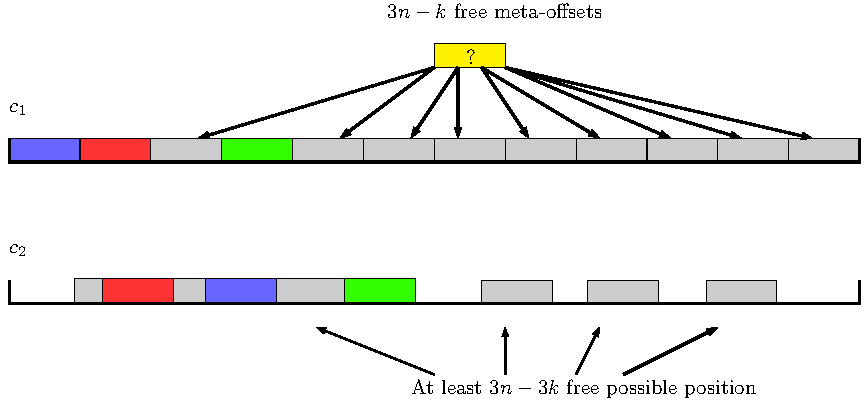
\includegraphics[width=0.7\textwidth]{Chapitre4PAZL/ex3nt.pdf}
      \end{center}
      \caption{Meta offsets used in the first and second period, when scheduling the $i+1^{th}$ datagram in \metaoffset. There is already 3 datagram in $S$ (in red, blue and green), and the meta offsets available for the yellow datagram are represented in grey.}
      \label{fig:metaoffset}
      \end{figure}

  
This algorithm, contrarily to the previous one, may work well, even for loads higher than $1/3$.
In fact, experimental data in Section~\ref{sec:perf_large} suggest that the algorithm finds a solution when the load is less than $1/2$.

%The method of this section is described in~\cite{dominique2018deterministic} and it achieves the same bound on the load using a different method. It is recalled here to help understand several algorithms in the article.
%The idea is to restrict the possible offsets at which datagrams can be scheduled. It seems counter-intuitive, since it decreases artificially the number of available offsets to schedule new datagrams. However, it allows reducing the number of forbidden offsets for unscheduled datagrams. A \textbf{meta-offset} is an offset of value $i\tau$,
%with $i$ an integer from $0$ to $P / \tau$. We call \metaoffset the greedy algorithm which works as \firstfit, but consider only meta-offsets when scheduling datagrams. 


%\begin{theorem}[Proposition 3 of~\cite{dominique2018deterministic}]
%\metaoffset solves \pma positively on instances of load less than $1/3$.
%\end{theorem}

A naive implementation of \metaoffset is in $O(n P/\tau)$, while \firstfit is in $O(nP)$.
However, it is not useful to consider every possible (meta-)offset at each step. By maintaining
a list of positions of scheduled datagrams in first and second period, both algorithms can be implemented in $O(n^2)$ ($n$ is the number of routes).


\subsection{Compact Tuples}\label{sec:compacttuple}

We present in this section a family of greedy algorithms which solve \pma positively for larger loads. We try to combine the good properties of the two previous algorithms: the compactness of the assignments produced by \firstfit and the absence of collision in the first period of \metaoffset. The idea is to schedule several datagrams at once, using meta-offsets, to maximize the compactness of the obtained solution. We first describe the algorithm which schedules pairs of datagrams and then explain quickly how to extend it to any tuples of datagrams.


We now introduce Lemma~\ref{lemma:multiple} to assume $P = m\tau$ and we use it until the end of the section. This hypothesis makes the analysis of algorithms based on meta-offsets simpler and tighter. The load increases from $\lambda = n \tau / P$ to at most $\lambda (1 + 1/m)$: the difference is less than $1/m < 1/n$, thus very small for most instances. The transformation of Lemma~\ref{lemma:multiple} does not give a bijection between assignments of both instances but only an injection, which is enough for our purpose. 

\begin{lemma}\label{lemma:multiple}
Let $I$ be an instance of \pma with $n$ datagrams of size $\tau$, period $P$ and $m = P / \tau$. There is an instance $I'$ with $n$ datagrams of size $\tau'$ and period $P'= m\tau'$ such that any assignment of $I'$ can be transformed into an assignment of $I$ in polynomial time.
\end{lemma}
\begin{proof}
Fig.~\ref{fig:multipleperiod} illustrates the reductions we define in this proof on a small instance.
Let $P = m \tau + r$ with $r \leq \tau$. We define the instance $I'$ as follows: $P' = mP$, $\notationdelay_{i}' = m \notationdelay_i$ and $\tau' = m \tau + r$. With this choice, we have $P' = m(m \tau + r) = m \tau'$.
Consider an assignment $A'$ of the instance $I'$.
If we let $\tau'' = m\tau$, then $A'$ is also an assignment for $I'' = (P',\tau'',(\notationdelay_{0}',\dots,\notationdelay_{n-1}'))$. Indeed, the size of each datagram, thus the intervals of time used in the first and second period begin at the same position but are shorter, which cannot create collisions. We then use a compactification procedure on $A'$ seen as an assignment of $I''$,
with size of datagrams multiple of $m$ (see Proposition~\ref{prop:compactification} for a similar compactification). W.l.o.g., the first datagram is positioned at offset zero. The first time it uses in the second period is a multiple of $m$ since its delay is by construction a multiple of $m$. Then, all other datagrams are translated to the left by removing increasing values to their offsets, until there is a collision. It guarantees that some datagram $j$ is in contact with the first one on the first or second period. It implies that either $A'(j)$ or $A'(j)+\notationdelay_j \mod P'$ is a multiple of $m$ and since $\notationdelay_j$ is a multiple of $m$, then both $A'(j)$ and $A'(j)+\notationdelay_j \mod P'$ are multiples of $m$. This procedure can be repeated until we get an assignment $A''$ to $I''$, such that all positions of datagrams in the first and second period are multiples of $m$. Finally, we define $A$ as $A(i) = A''(i)/m$ and we obtain an assignment of $I$. 
\end{proof}

\begin{figure}
 \begin{center}
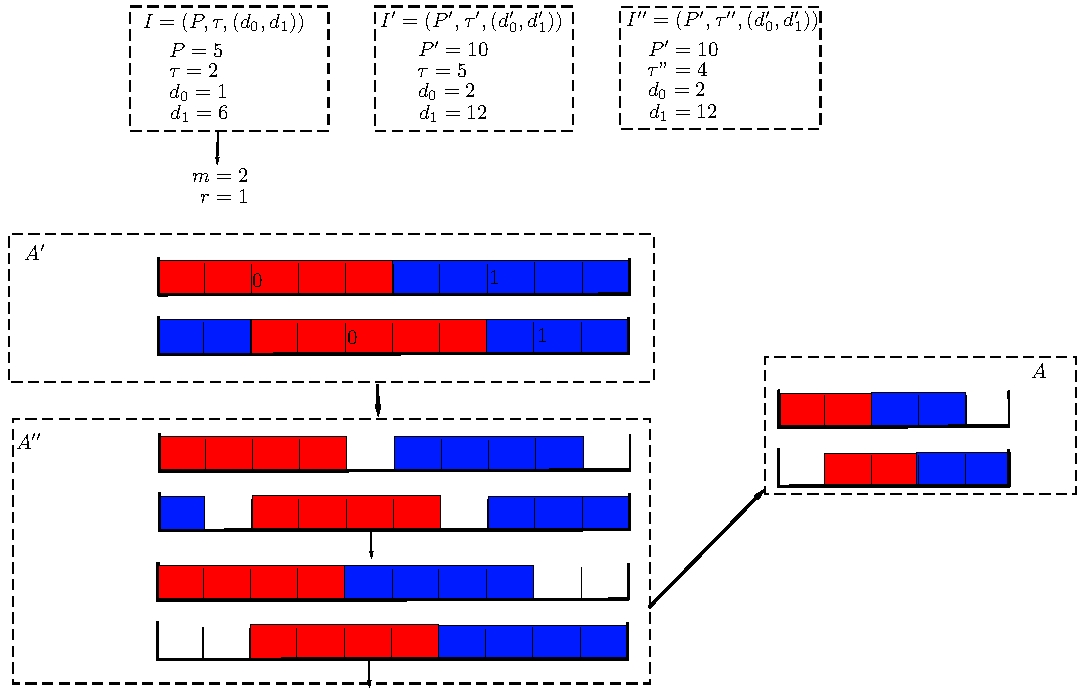
\includegraphics[scale=0.75]{Chapitre4PAZL/multipleperiod}
\end{center}
\caption{Transformation from $A''$ to $A$}
\label{fig:multipleperiod}
\end{figure}


We are interested in the remainder modulo $\tau$ of the delays, let $\notationdelay_i = \notationdelay_{i}'\tau + r_i$ be the Euclidean division of $\notationdelay_i$ by $\tau$. We assume, from now on, that \emph{datagrams are sorted by increasing $r_i$}.
A \textbf{Compact pair}, as shown in Fig.~\ref{fig:compactpair} is a pair of datagrams $(i,j)$ with $i < j$ that can be scheduled using meta-offsets such that $A(i) + (\notationdelay'_i+1)\tau = A(j) + \notationdelay'_j\tau$, i.e. $j$ is positioned less than $\tau$ unit of times after $i$ in the second period.
The \textbf{gap} between $i$ and $j$ is defined as  $g = \notationdelay_{i}' + 1 - \notationdelay_{j}' \mod m$, it is the distance in meta offsets between $i$ and $j$ in the first period. By definition, we can make a compact pair out of $i$ and $j$, if and only if their gap is not zero.

\begin{figure}[h]
\begin{center}



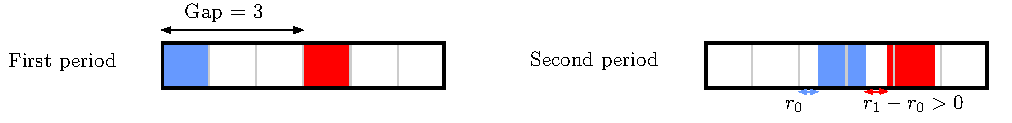
\includegraphics[scale=0.7]{Chapitre4PAZL/compact_pair}
\end{center}
\caption{A compact pair scheduled using meta-offsets, with $d'_0 = 2$ and $d'_0 = 0$}
\label{fig:compactpair}
\end{figure}

\begin{lemma}\label{lemma:pair_find}
Given three datagrams of delay $\notationdelay_{1}$, $\notationdelay_{2}$ and $\notationdelay_{3}$, two of them form a compact pair. 
\end{lemma}
\begin{proof}
If the first two datagrams or the first and the third datagram form a compact pair,
then we are done. If not, then by definition $\notationdelay_{1}' = 1 + \notationdelay_{2}' = 1 + \notationdelay_{3}'$. Hence, datagrams $2$ and $3$ have the same delay and form a compact pair of gap $1$.
\end{proof}

Let \compactpair be the following greedy algorithm: From the datagrams in order
of increasing $r_i$, a sequence of at least $n/3$ compact pairs is built using Lemma~\ref{lemma:pair_find}. Pairs are scheduled in the order they have been built using meta-offsets. If at some point all compact pairs are scheduled or the current one cannot be scheduled, the remaining datagrams are scheduled as in \metaoffset. The analysis of \compactpair relies on the evaluation of the number of forbidden meta-offsets. In the first phase of \compactpair, one should evaluate the number of forbidden offsets when scheduling a compact pair, that we denote by $Fmo_2(A)$. In the second phase, we need to evaluate $Fmo(A)$. When scheduling a datagram in the second phase, a scheduled compact pair only forbids \emph{three} meta-offsets in the second period. If datagrams in a pair are scheduled independently, they forbid \emph{four} meta-offsets, which explains the improvement from \compactpair. We first state a simple lemma, whose proof can be read from Fig.~\ref{fig:forbidenmeta}, which allows bounding $Fmo_2(A)$.

\begin{lemma}\label{lemma:pair_forbid}
A compact pair already scheduled by \compactpair forbids at most four meta-offsets in the second period to another compact pair when scheduled by \compactpair.
\end{lemma}

\begin{figure}
\begin{center}
\includegraphics[scale=0.7]{Chapitre4PAZL/pairforbiden}
\end{center}

\caption{Meta offsets forbidden by a scheduled compact pair (in blue) when scheduling another compact pair (in red)} 
\label{fig:forbidenmeta}
\end{figure}
\begin{theorem}
\compactpair solves \pma positively on instances of load less than
$3/8$.
\end{theorem}
\begin{proof}
Let $n_2$ be the number of compact pairs scheduled in the first phase. When scheduling a new pair, the position of the $2n_2$ datagrams on the first period forbid $4n_2$ offsets for a compact pair. Indeed, each scheduled datagram can collide
with each of the two datagrams which form a compact pair. On the second period, we can use Lemma~\ref{lemma:pair_forbid} to bound the number of forbidden offsets by $4n_2$. 
Hence, we have established that during the first phase, the partial solution $A$
satisfies $Fmo_2(A) \leq 8n_2$. This first phase continues while there are available offsets for compact pairs, which is guaranteed when $Fmo_2(A) \leq m$, that is while $n_2 \leq m/8$. Hence, we assume that $n_2 = m/8$.

In the second phase, a compact pair forbids $3$ meta offsets in the 
second period and $2$ in the first. Hence, if we let $n_1$ be the number of datagrams scheduled in the second phase to build partial assignment $A$, we have $Fmo(A) \leq n_2*5 + n_1*3$. 
\compactpair can always schedule datagrams when $Fmo(A)$ is less than $m$, which is implied by $n_2*5 + n_1*3 \leq m$.
Solving this equation, we obtain that $n_1 \geq \frac{m}{8}$ thus the number of datagrams scheduled is at least $2n_2 + n_1 \geq \frac{3}{8}m$. Assuming there are exactly $\frac{3}{8}m$ datagrams to schedule, then $\frac{2m}{8}$ datagrams are scheduled as compact pairs. It is two third of the $\frac{3}{8}m$ datagrams, hence Lemma~\ref{lemma:pair_find} guarantees the existence of enough compact pairs. Therefore, an assignment is always produced when the load is less or equal to $\frac{3}{8}$.
\end{proof}

\compactpair can be improved by forming compact tuples instead of compact pairs.
A compact $k$-tuple is a sequence of datagrams $i_1 < \dots < i_k$ (with $r_{i_1},\dots,r_{i_k}$ increasing), for which meta-offsets can be chosen so that, there is no collision, the datagrams in the second period are in order $i_1,\dots,i_k$ and for all $l$, $A(i_l) + (\notationdelay'_{i_l} + 1)\tau = A(i_{l+1}) + \notationdelay'_{i_{l+1}}\tau$.
The algorithm \texttt{Compact k-tuples} works by scheduling compact $k$-tuples
using meta offsets while possible, then scheduling compact $k-1$-tuples and so on until $k=1$.


\begin{lemma}\label{lemma:uple_find}
Given $k + k(k-1)(2k-1)/6$ datagrams, $k$ of them always form a compact $k$-tuple and we can find them in polynomial time. 
\end{lemma}
\begin{proof}
We prove the property by induction on $k$. We have already proved it for $k=2$ in Lemma~\ref{lemma:pair_find}.
Now assume that we have found $C$ a compact $(k-1)$-tuple in the first $(k-1)^3/3$
datagrams. Consider the next $(k-1)^2 + 1$ datagrams. If $k$ of them have the same delay modulo $\tau$,
then they form a compact $k$-tuple and we are done. Otherwise, there are at least $k$ different values modulo $\tau$
in those $(k-1)^2 + 1$ datagrams. Each element of the compact $(k-1)$-tuple forbids one value for the delay modulo $\tau$ of a new $k$th element in the tuple. By pigeonhole principle, one of the $k$ datagrams with distinct delays modulo $\tau$ can be used to extend $C$. We have built a compact $k$-tuple from at most $(k-1) + (k-1)(k-2)(2k-3)/6 + (k-1)^2 + 1$ datagrams.
It is equal to $k + k(k-1)(2k-1)/6$ which proves the induction.
\end{proof}


\begin{theorem}\label{th:k-tuples}
\texttt{Compact 8-tuples} always solves \pma positively on instances of load less than $4/10$, for instances with $n \geq 220$.
\end{theorem}
\begin{proof}
We need the following fact, which generalizes Lemma~\ref{lemma:pair_forbid}: A $k$-tuples forbids $k+j+1$ offsets in the second period when scheduling a $j$-tuple. %If the remainder of the datagrams in the $j$-tuples are larger than the remainder in the $k$-tuples, it forbids $k+j$ datagrams only.
It enables us to compute a lower bound on the number of scheduled $i$-tuples for $i$ equal $k$ down to $1$ by bounding $Fmo_i(A)$, the number of forbidden meta-offsets when placing $i$-tuple in the algorithm.
If we denote by $n_i$ the number of compact $i$-tuples scheduled by the algorithm,
we have the following equation:  $$ Fmo_i(A) \leq \displaystyle{\sum_{j=i}^k n_j(j*i + j + i+ 1)}.$$
The equation for $n_1$ is slightly better: 
$$ Fmo(A) \leq \displaystyle{\sum_{j=1}^k n_j(2j + 1)}.$$
A bound on $n_i$ can be computed, using the fact that $A$ can be extended while $Fmo_i(A) < m$. 
Lemma~\ref{lemma:uple_find} ensures there are enough compact $k$-tuples, when $n - \sum_{j \leq i \leq 8} n_j$ is larger than $i + i(i-1)(2i-1)/6$. 
A numerical computation of the $n_i$'s shows that \texttt{Compact 8-tuples} always finds an assignment when the load is less than $4/10$ and for $n \geq 220$.
\end{proof}

Th.~\ref{th:k-tuples} is obtained for $k=8$. Taking arbitrary large $k$ and using refined bounds on $Fmo_i(A)$ is not enough to get an algorithm working for a load of $41/100$ (and it only works from larger $n$).

The code computing the $n_i$ can be found on~\cite{webpage}.
To make \texttt{Compact 8-tuples} work, there must be at least $220$ datagrams to
produce enough compact $8$-tuples in the first phase. It is not a strong restriction for two reasons. First, the bound of Lemma~\ref{lemma:uple_find} can be improved, using a smarter polynomial time algorithm to find compact tuples, which better takes into account repetitions of values and compute the compact tuples in both directions. Second, on random instances, the probability that $k$ datagrams do not form a compact $k$-tuples is low, and we can just build the tuples greedily. Therefore, for most instances, forming compact $k$-uples is not a problem and in practice \texttt{Compact 8-tuples} works even for small $n$.



We describe here a last algorithm called \compactfit, which is a simpler variant of the previous one. The idea is, as for \compactpair, to combine the absence of collision on the first period of \metaoffset and the compactness of assignments given by \firstfit.
The datagrams are ordered by increasing remainder of delay modulo $\tau$, and each datagram is scheduled so that 
it extends an already scheduled compact tuples. In other words, it is scheduled using meta offsets, so that using one less as a meta-offset for some datagram creates a collision in \emph{the second period}. If it is not possible to schedule the datagram in that way, the first possible meta-offset is chosen. This algorithm is designed to work well on random instances. Indeed, it 
is easy to evaluate the average size of the created compact tuples, and from that, to prove that \compactfit works with high probability when the load is strictly less than $1/2$.
\begin{figure}[h]
 \begin{center}
\includegraphics[scale=1]{Chapitre4PAZL/compactfit}
\end{center}
\caption{Execution of \compactfit creating two compact pairs with $P=12$ and $\tau =2$}
\label{fig:compactfit}
\end{figure}
Figure~\ref{fig:compactfit} shows how \compactfit builds an assignment from a given instance. The datagrams are ordered by increasing remainder of delay modulo $\tau$. A compact pair is built with datagrams $0$ and $1$. Datagram $2$ cannot increase the size of the compact pair, it so creates a new tuple, completed by datagram $3$



\subsection{Compact Assignment}

In this section, we show how every bufferless assignment can be put into a canonical form.
We use that form to design an algorithm solving \pma in fixed parameter tractable time ($\FPT$), with parameter $n$ the number of routes (for more on parametrized complexity see~\cite{downey2012parameterized}). This is justified since $n$ is small in practice, from $10$ to $20$ in our settings, and the other parameters such as $P$, $\tau$ or the weights are large.

Let $({\cal R},\omega)$ be a star routed network and let $A$ be a bufferless $(P,\tau)$-periodic assignment.
We say that that $A$ is \textbf{compact} if there is a route $r_0 \in \cal{R}$ such that the following holds: for all subsets $S\subset \cal{R}$ with $r_0 \notin S$, the bufferless assignment $A'$, defined by $A'(r) = A(r) - 1 \mod P$ if $r \in S$ and $A(r)$ otherwise, is not valid. In other words, an assignment is compact if for all routes $r$ but one, $A(r)$ cannot be reduced by one, that is either in the first or the second period, there is a route $r'$ using the tics just before $A(r)$. See Figure~\ref{fig:compact} for an example of a compact assignment, obtained by the procedure of the next proposition. 
  \begin{figure}
      \begin{center} 
      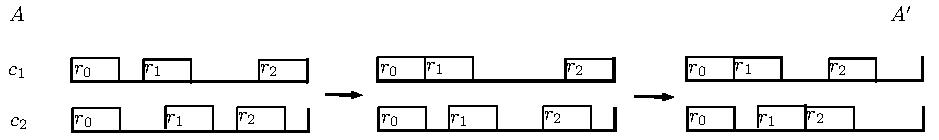
\includegraphics[width=\textwidth]{Chapitre4PAZL/compacttoassignment.pdf}
      \end{center}
      \caption{Transformation of a bufferless assignment $A$ into a compact assignment $A'$, following the process of Proposition~\ref{prop:compactification}}
      \label{fig:compact}
      \end{figure}
\begin{proposition}\label{prop:compactification}
Let $N = ({\cal R}, \omega)$ be a star routed network. If there is a $(P,\tau)$-periodic bufferless assignment of $N$, then there is a compact $(P,\tau)$-periodic assignment of $N$.
\end{proposition}
\begin{proof}
Consider $A$ a $(P,\tau)$-periodic bufferless assignment of $N$.
We describe an algorithm which builds a sequence $(r_0,\dots,r_{n-1})$ and a sequence  
$A_i$ of valid bufferless assignments. We denote by $COMP_i = \{ r_j \mid j < i\}$

Let $r_0$ be an arbitrary route of ${\cal R}$ and $A_0 = A$. For $i = 1$ to $n$, we choose $r_i$ as follows.
Let $A_{i} = A_{i-1}$. While there is no collision, for all routes $r \in {\cal R} \setminus COMP_i$, let $A_i(r) = A_i(r) - 1$. Then choose any route $r$ in ${\cal R} \setminus COMP$ such that setting $A_i(r) = A_i(r-1)$ creates a collision and let $r_i = r$. By construction $A_i$ is a valid bufferless assignment, since it is modified only when no collision is created.

We prove by induction on $i$, that $A_i$ is compact when restricted to $COMP_{i+1}$.
For $i = 0$, $|COMP_1| = 1$ and the property is trivially satisfied. Let us consider $A_i$,
by induction hypothesis, since the offsets of routes in $COMP_{i}$ are not modified at step $i$ of the algorithm, $A$ is compact when restricted to $COMP_{i}$. 

 Consider $S \subseteq COMP_i$ which does not contain $r_0$. If $S$ contains
an element of $COMP_{i}$, then $S \setminus {r_i}$ is not empty and by compactness we cannot decrement all offsets of $S\setminus {r_i}$ without creating a collision. The same property is true for $S$. If $S = \{r_i\}$, then by construction of $r_i$ by the algorithm, removing one from $A_i(r_i)$ creates a collision. Hence,
$A_i$ is compact restricted to $COMP_{i+1}$, which proves the induction and the proposition.
\end{proof}

We now present an algorithm to find a $(P,\tau)$-periodic assignment by trying all compact assignments.

\begin{theorem}\label{th:FPT}
$\pma \in \FPT$ over star routed networks when parametrized by the number of routes.
\end{theorem}
\begin{proof}
Let $N = ({\cal R},\omega)$ be a canonical star routed network and let $P$ be the period and $\tau$ the size of a datagram. First, remark that for a given assignment and a route $r$ with offset $o_r$, by removing $o_r$ to all offsets, we can always assume that $o_r = 0$. By this remark and Proposition~\ref{prop:compactification}, we need only to consider all \emph{compact assignments} with an \emph{offset $0$} for the route $r_0$. We now evaluate the number of compact assignments and prove that it only depends on $n$ the number of routes to prove the theorem.

 We describe a way to build any compact assignment $A$ by determining its offsets one after the other, which gives a bound on their number and an algorithm to generate them all. We fix an arbitrary total order on ${\cal R}$. Let $r_0$ be the smallest route of $\cal{R}$, its offset is set to $0$ and we let $S = \{r_0\}$,
 $S_1 = \{r_0\}$ and $S_2 = \{r_0\}$. $S$ represent the routes whose offsets are fixed, 
 offsets of unscheduled routes are chosen so that they follow a route of $S_1$ in the first period or a route of $S_2$ in the second period.

 At each step, we add an element to $S$: let $r$ be the smallest element of $S_1$, if it is non empty. Then, select any route $r' \in {\cal R} \setminus S$ 
 such that $o_{r'} = o_{r} + \tau$ does not create collision (by construction $o_{r'} = o_{r} + \tau - 1$ does create a collision in the first period). Then, we update the sets as follows:
 $S = S \cup \{r'\}$, $S_1 = S_1 \setminus \{r\} \cup \{r'\}$ and $S_2 = S_2 \cup \{r'\}$. If 
 $S_1$ is empty, $r$ is smallest element of $S_2$, and we set $o_{r'} = o_{r} + \tau + \omega(r,c_2) - \omega(r',c_2)$.
 We can also remove $r$ from $S_1$ (or from $S_2$ if $S_1$ is empty) without adding any element to $S$. Remark that the value of the offset of the route added to $S$ is entirely determined by the values of the offsets of the routes in $S$.

 Now, remark that any compact assignment can be built by this procedure, if the proper choice of element to add is made at each step. Hence, this process generates all compact assignments. We now bound the number of compact assignments it can produce. Remark that, when $|S| = i$, we can add any of the $n-i$ routes in ${\cal R} \setminus S$ to $S$. Hence, the number of sequences of choices of routes to add is $n!$ (but some of these sequences can fail to produce a valid assignment). We have not yet taken into account the steps at which an element is removed from either $S_1$ or $S_2$, without adding something to $S$. At each step of the algorithm, we can remove an element or not, there are at most $2n$ steps in the algorithm, hence there are at most $4^n$ sequences of such choices during the algorithm. As a conclusion, there are at most $4^nn!$ compact assignments.

The algorithm to solve \pma builds every possible compact assignment in the incremental manner described here, and tests at each step whether, in the built partial assignment, there is a collision, which can be done in time linear in the size of $N$. Therefore $\pma \in \FPT$.
\end{proof}


We call the algorithm described in Theorem~\ref{th:FPT} \textbf{E}xhaustive \textbf{S}earch of \textbf{C}ompact \textbf{A}ssignments or \ESCA. The complexity of \ESCA is in $O(4^n n!)$. While a better analysis of the number of compact assignments could improve this bound, the simple star routed networks with all arcs of weights $0$ has $(n-1)!$ compact assignments. Hence, to improve significantly on \ESCA, one should find an even more restricted notion of bufferless assignment than compact assignment.

To make \ESCA more efficient in practice, we make cuts in the search tree used to explore all compact assignments. Consider a set $S$ of $k$ routes whose offsets have been fixed at some point in the search tree. We consider the times used by these routes in the first period. It divides the period into $[(a_0,b_0), \dots, (a_{k-1},b_{k-1})]$ where the intervals $(a_i,b_i)$ are the times not used yet in the first period. Therefore at most $\displaystyle{ \sum_{i=0}^{k-1} \lfloor(b_{i} -a_i)/\tau\rfloor}$ routes can still send a datagram through the first period. If this value is less than $n - k$, it is not possible to create a compact assignment by extending the current one on $S$ and we backtrack in the search tree. The same cut is also used for the second period. These cuts rely on the fact that the partial assignment is wasting bandwidth by creating intervals which are not multiples of $\tau$. It helps with instances of large load, which are also the hardest to solve.


\subsection{Experimental Results} \label{sec:perf_large}

\subsubsection{Cloud-Ran Parameters}\label{sec:pazlcran}
In this section, the performance on random instances of the algorithms presented in Sec.~\ref{sec:large} is experimentally characterized.
%rs are some reference to realistic parameters and the objective here is to evaluate our algorithm performances.

  The defaults parameters of experiments of this section are derived from the C-RAN context: a tic correspond to the sending time of $64$ Bytes of data on links of bandwidth $10$~Gbps. The datagrams are of size $1$~Mbit, which corresponds to $2,500$ tics.% The number of routes is set to $n = 8$ in most experiments.
   In the Cloud-RAN problem, the period fixed by the protocol HARQ correspond to $21,000$ tics. This means that a network with $8$ routes is loaded at $95\%$, which seems unrealistic and cannot be solved for \pma, as we experimentally show it in this section. Nevertheless, we choose these parameters as a realistic reference and we modify them in order to evaluate our algorithm performances.


     All experiments are done on synthetic data generated randomly. We generate the physical fronthaul
     network represented in Figure~\ref{fig:star} of Chapter~\ref{chap:model}. We consider routes which are shorter than $\tau$: a datagram cannot be contained completely in a single arc which is common in our applications. We generate random star routed networks, by drawing uniformly at random the weights of the arcs in $[700]$. This corresponds to links of the networks of less than $5$km between a BBU and an RRH. Then, the corresponding canonical star routed network is built from the generated fronthaul and the algorithms tested on it. This process is mostly equivalent to drawing the delays randomly in $[1400]$.

     We consider the following algorithms:
\begin{itemize}
  \item \shortestlongest
  \item \firstfit
  \item \metaoffset
  \item \compactpair
  \item \compactfit
  \item \greedyuniform, the algorithm introduced and analyzed in Section~\ref{sec:small}, used for arbitrary $\tau$
  \item \exactresolution 
\end{itemize}

%Since the delays are drawn in $\tau$, the algorithms based on meta-offsets works without the transformation of Lemma~\ref{lemma:multiple}. Indeed, since we consider only the offsets that are multiples of $\tau$ in the first period, the tics corresponding to the remainder of $P mod \tau$ are naturally lost. Furthermore, by considering the last

     In the following experiments, we illustrate how well the algorithms work with regards to the load. To change the load, both parameters $\tau$ and $n$ are fixed and we modify the period $P$, which allows for a smooth control of the load and does not impact the execution time of the algorithms.
	   We generate $10,000$ random instances of \pma of load from $0.5$ to $1$. We represent, in Figure~\ref{fig:short}, the percentage of success of each algorithm as a function of the load. We make three experiments with $8$, $12$ and $16$ routes to understand the effect of the number of routes on the quality of our algorithms. A bound on the maximal success rate is given by \ESCA (exhaustive search) which always finds a solution if there is one. 

     The code in C is available on \cite{webpage} under a copyleft license. The code has been run on a standard $2016$ laptop with a $2.2$~Ghz Intel Core i5 and the sources are compiled with gcc version 7.5.0. All experiments on $8$ routes end in at most a few dozen seconds.



      \begin{figure}[H]
      \begin{center}
   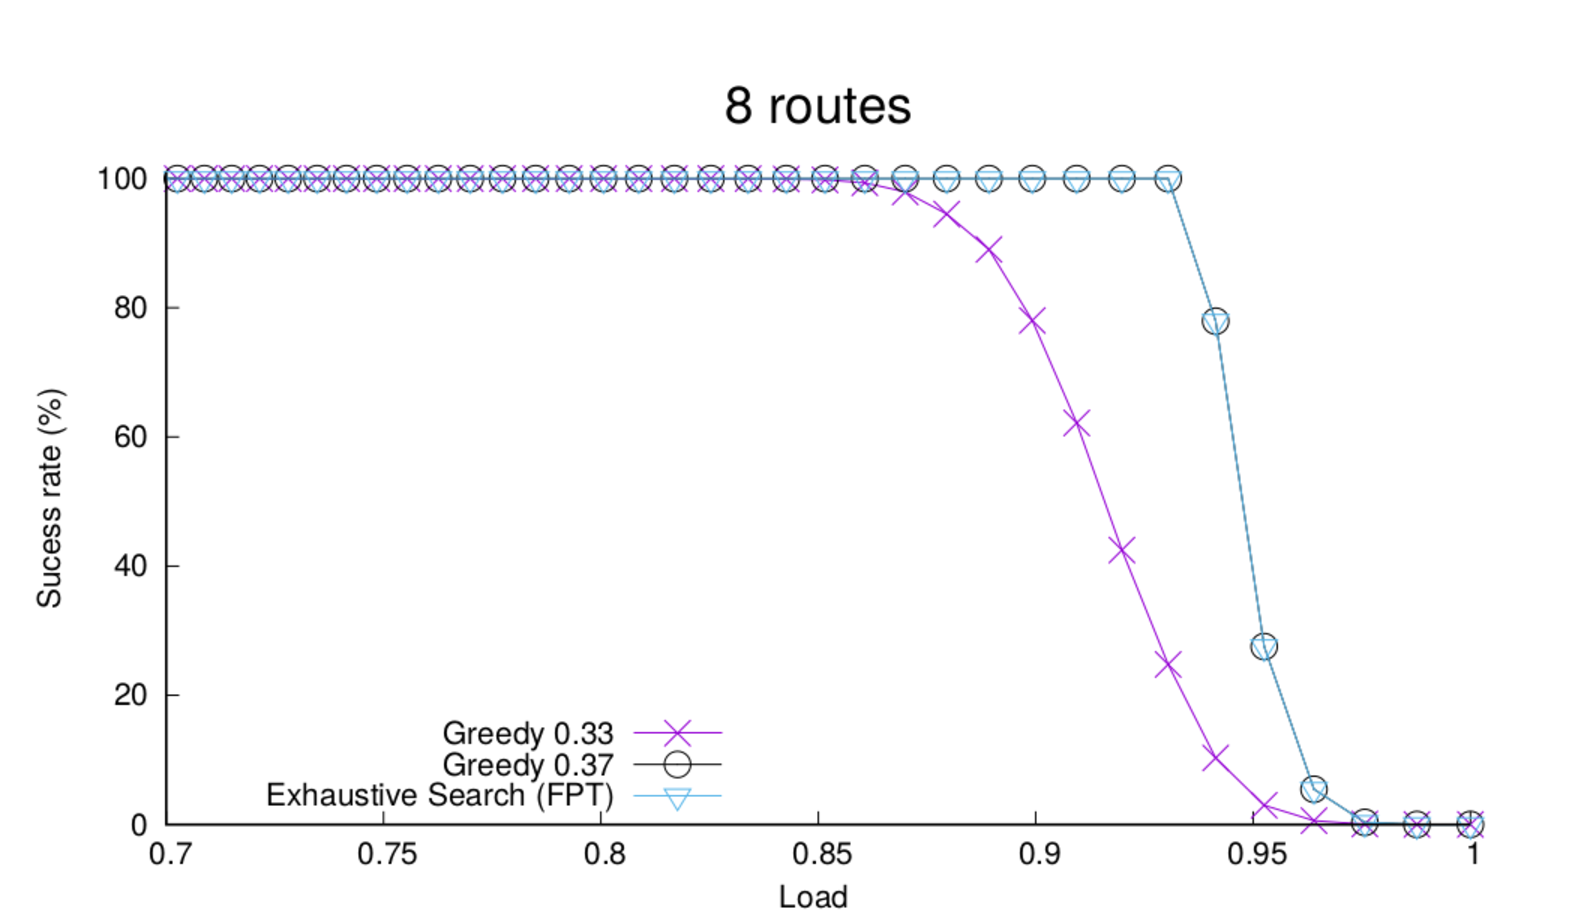
\includegraphics[width=0.45\textwidth]{Chapitre4PAZL/pazlshort8.pdf}
   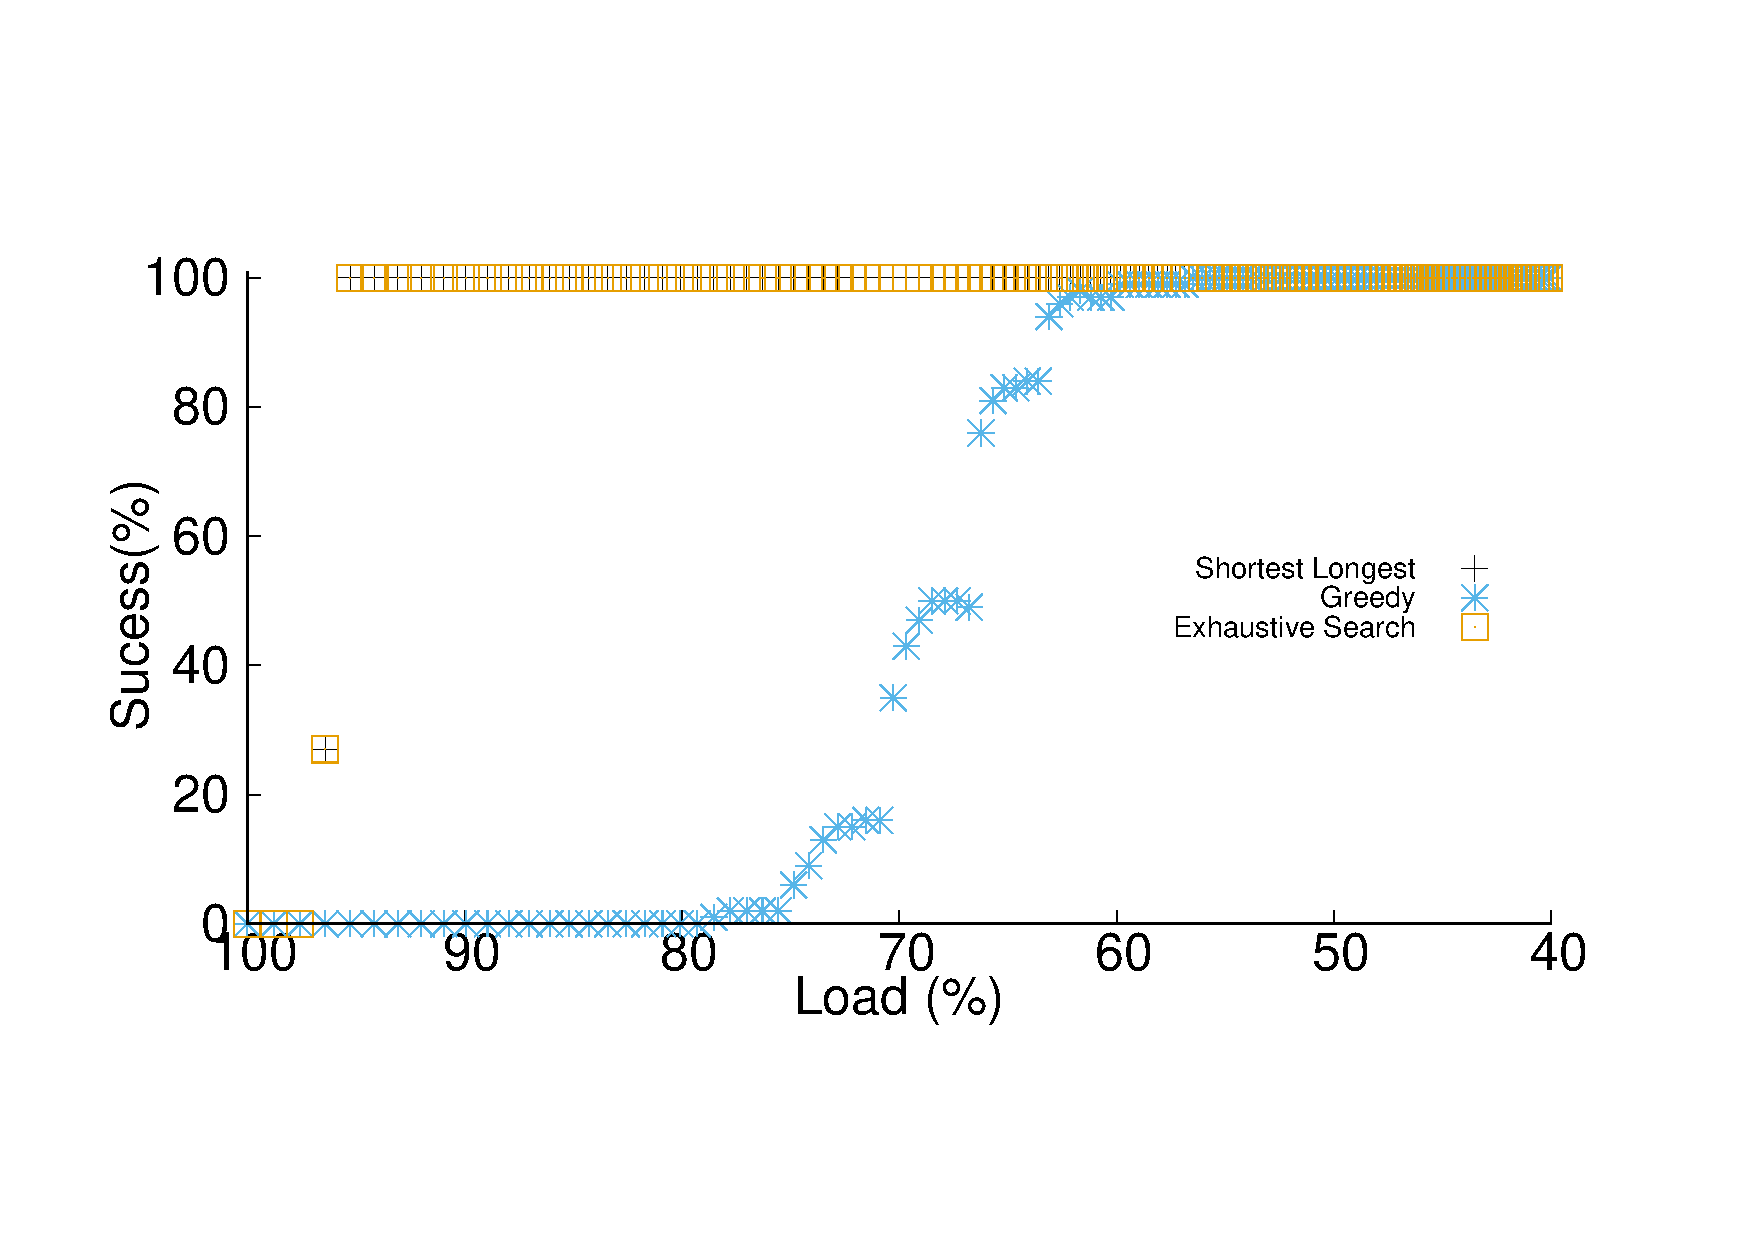
\includegraphics[width=0.45\textwidth]{Chapitre4PAZL/pazlshort12.pdf}

   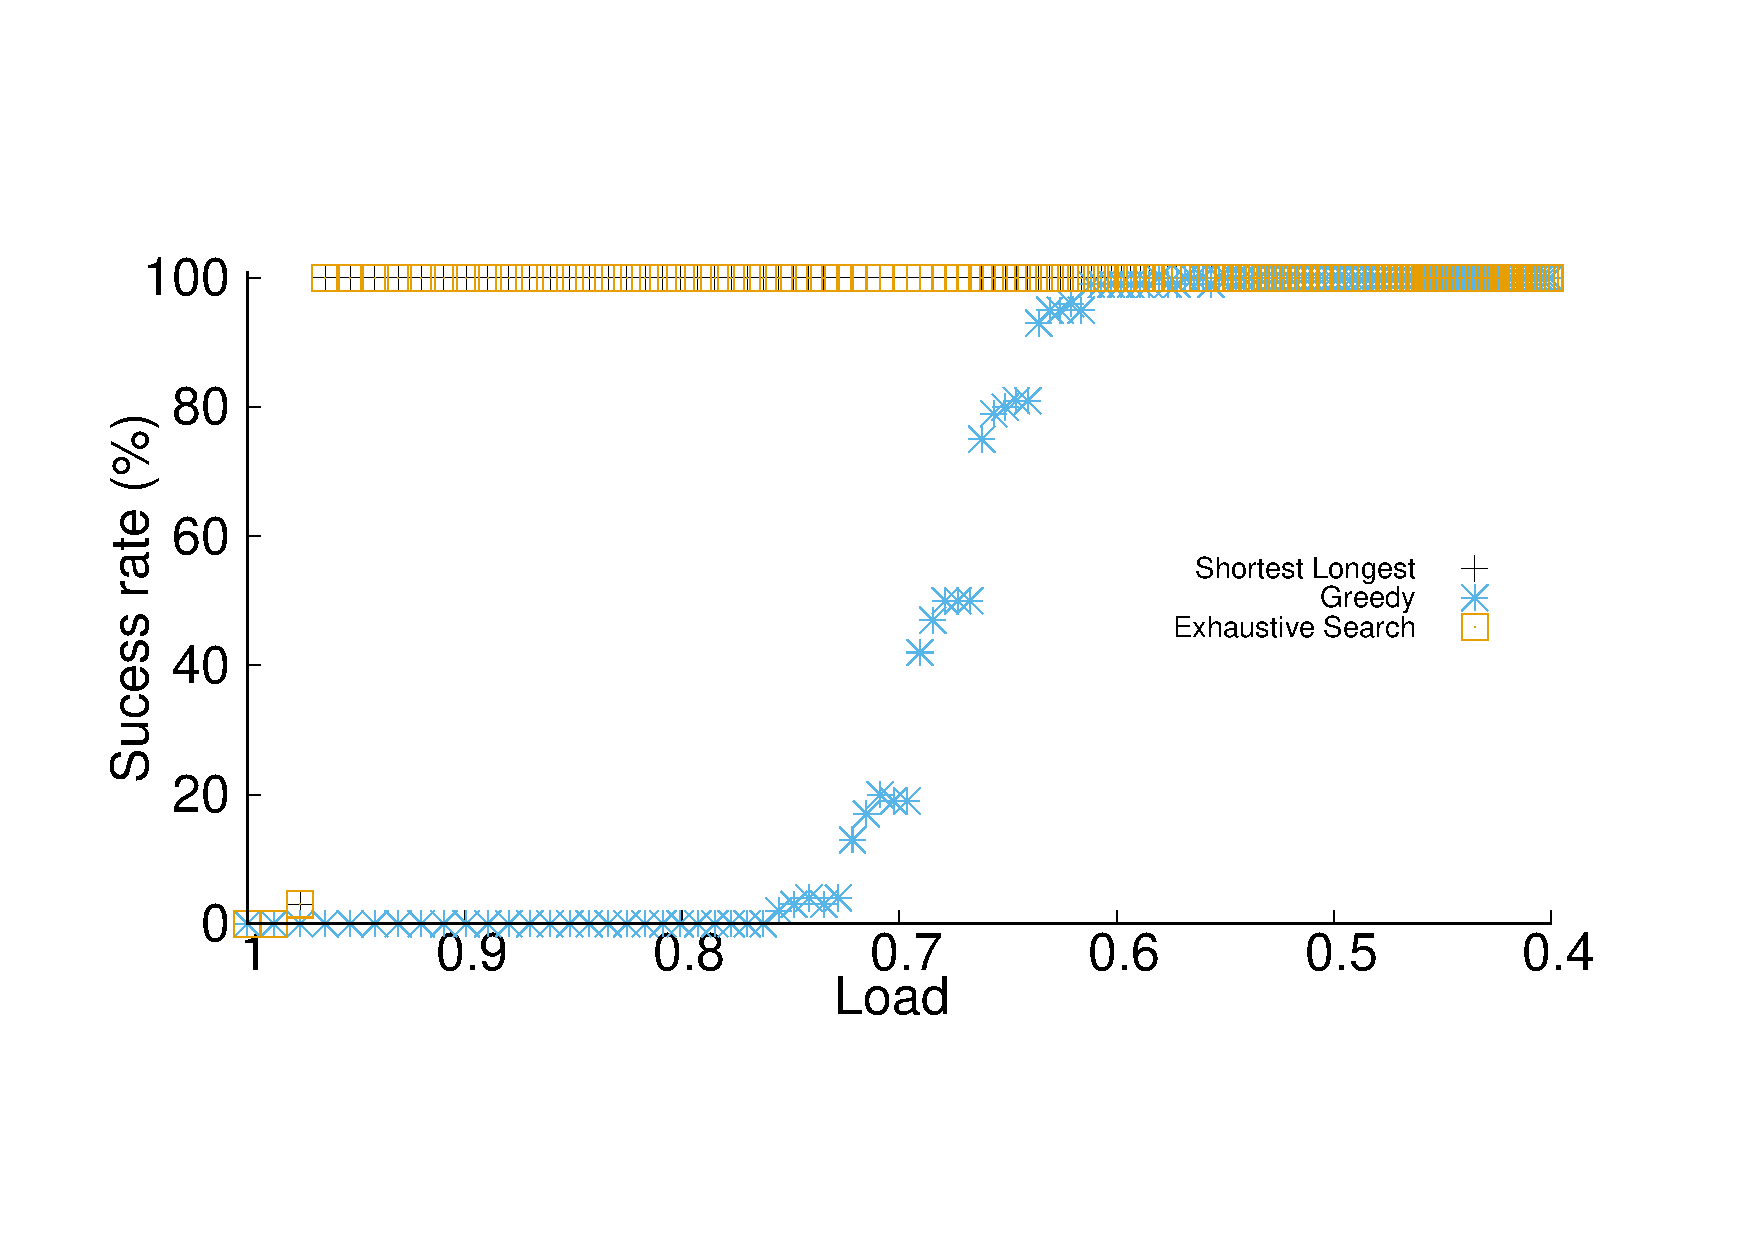
\includegraphics[width=0.45\textwidth]{Chapitre4PAZL/pazlshort16.pdf}
      \end{center}
      \caption{Success rate of three algorithms solving \pma, for short routes and $8$ routes (left), $12$ routes (right) and $16$ routes (middle)}\label{fig:short}
      \end{figure}

      First, we remark that \ESCA finds a solution even when the load is high. It justifies the idea to look for a bufferless assignment in this short routes regime. It seems that increasing the number of routes increases the success rate of \ESCA, meaning that the more the routes, the more instances have a bufferless assignment. 
      Second, remark that \shortestlongest is as good as the exhaustive search. While it was expected to be good with short routes (see Proposition~\ref{prop:SL}), it turns out to be optimal for all the random star routed networks we have tried. Therefore, we should use it in practical applications with short routes, instead of the exhaustive search which is much more computationally expensive. 
      Also, \compactpair and \compactfit have the same performances as \ESCA and \shortestlongest. This is not surprising when the routes are drawn on a lower range than $\tau$. Indeed, since we sort the routes by remainder modulo $\tau$  in \compactpair and \compactfit (which are just there values then), these two algorithms build the same assignment as \shortestlongest.

       \firstfit has also excellent performances ($100\%$ of success under loads lower to $0.8$). However, since we do not have strong theoretical results for this algorithms and it does not performs as well as \shortestlongest in this regime, it is not interesting to rely on it.

      \metaoffset and \greedyuniform both seem to always work when the load is less than $1/2$ and have a good probability to work up to a load of $2/3$, which is twice better than the theoretical bound. \metaoffset presents discontinuities in the probability of success at several loads, which seems to smooth out when the number of routes increases. It can be explained by the fact that \metaoffset becomes better when decreasing the load makes the number of available meta-offsets larger, which happens each time $\tau$ is added to the period (to decrease the load, the period is increased) and is more frequent when there are more routes.
      
      \greedyuniform and \metaoffset performances depend on the number of routes. The more routes there is, the lower the success rate. This is even clearer in experiment of Figure~\ref{fig:shortroutes} in the next section in which there is $100$ routes. Remember that \greedyuniform is an algorithm presented and analyzed in Section~\ref{sec:small}. This algorithm is designed for $\tau = 1$ and random delays and has no theoretical guarantee for arbitrary $\tau$ and small delay.
     



\subsubsection{Larger Route Number}\label{sec:pazlmanyroutes} 

After studying the C-RAN parameters, we want to experiment the performance of our algorithm with a larger number of routes and/or delays drawn in a larger interval.
We experiment with several periods and datagram sizes. For each set of parameters, we try every possible load by changing the number of datagrams and give the success rate of each algorithm. Notice that all algorithm except \ESCA are in polynomial time but are not always able to find a solution, depending on the load or the size of the routes. On the other hand, \ESCA finds a solution if it exists, but works in exponential time in $n$.
 The success rate is measured on $10000$ instances of \pma generated by drawing uniformly and independently the delays of each datagram in $[P]$ or $[\tau]$ for Figure~\ref{fig:shortroutes}. 


On a regular laptop, all algorithms terminates in less than a second when solving $10000$ instances with $100$ datagrams except \ESCA, whose complexity is exponential in the number of routes (but polynomial in the rest of the parameters). Hence, the optimal value of the success rate given by \ESCA is only available in the experiment with at most $10$ routes (the algorithm cannot compute a solution in less than an hour for twenty datagrams and high load). 
Note that while \firstfit, \compactpair, \metaoffset, \compactfit all run in almost the same time,
\greedyuniform seems to be three times longer than the other algorithms to run on instances with $100$ datagrams. It is expected since, at each step, it must find all available offsets to draw one uniformly at random instead of just choosing one.

In the following experiments, since Lemma~\ref{lemma:multiple} explains how to transform any instance into one with  $P = m\tau$, we chose for simplicity that $P = m\tau$.

\begin{minipage}[c]{.49\linewidth}

\begin{center}
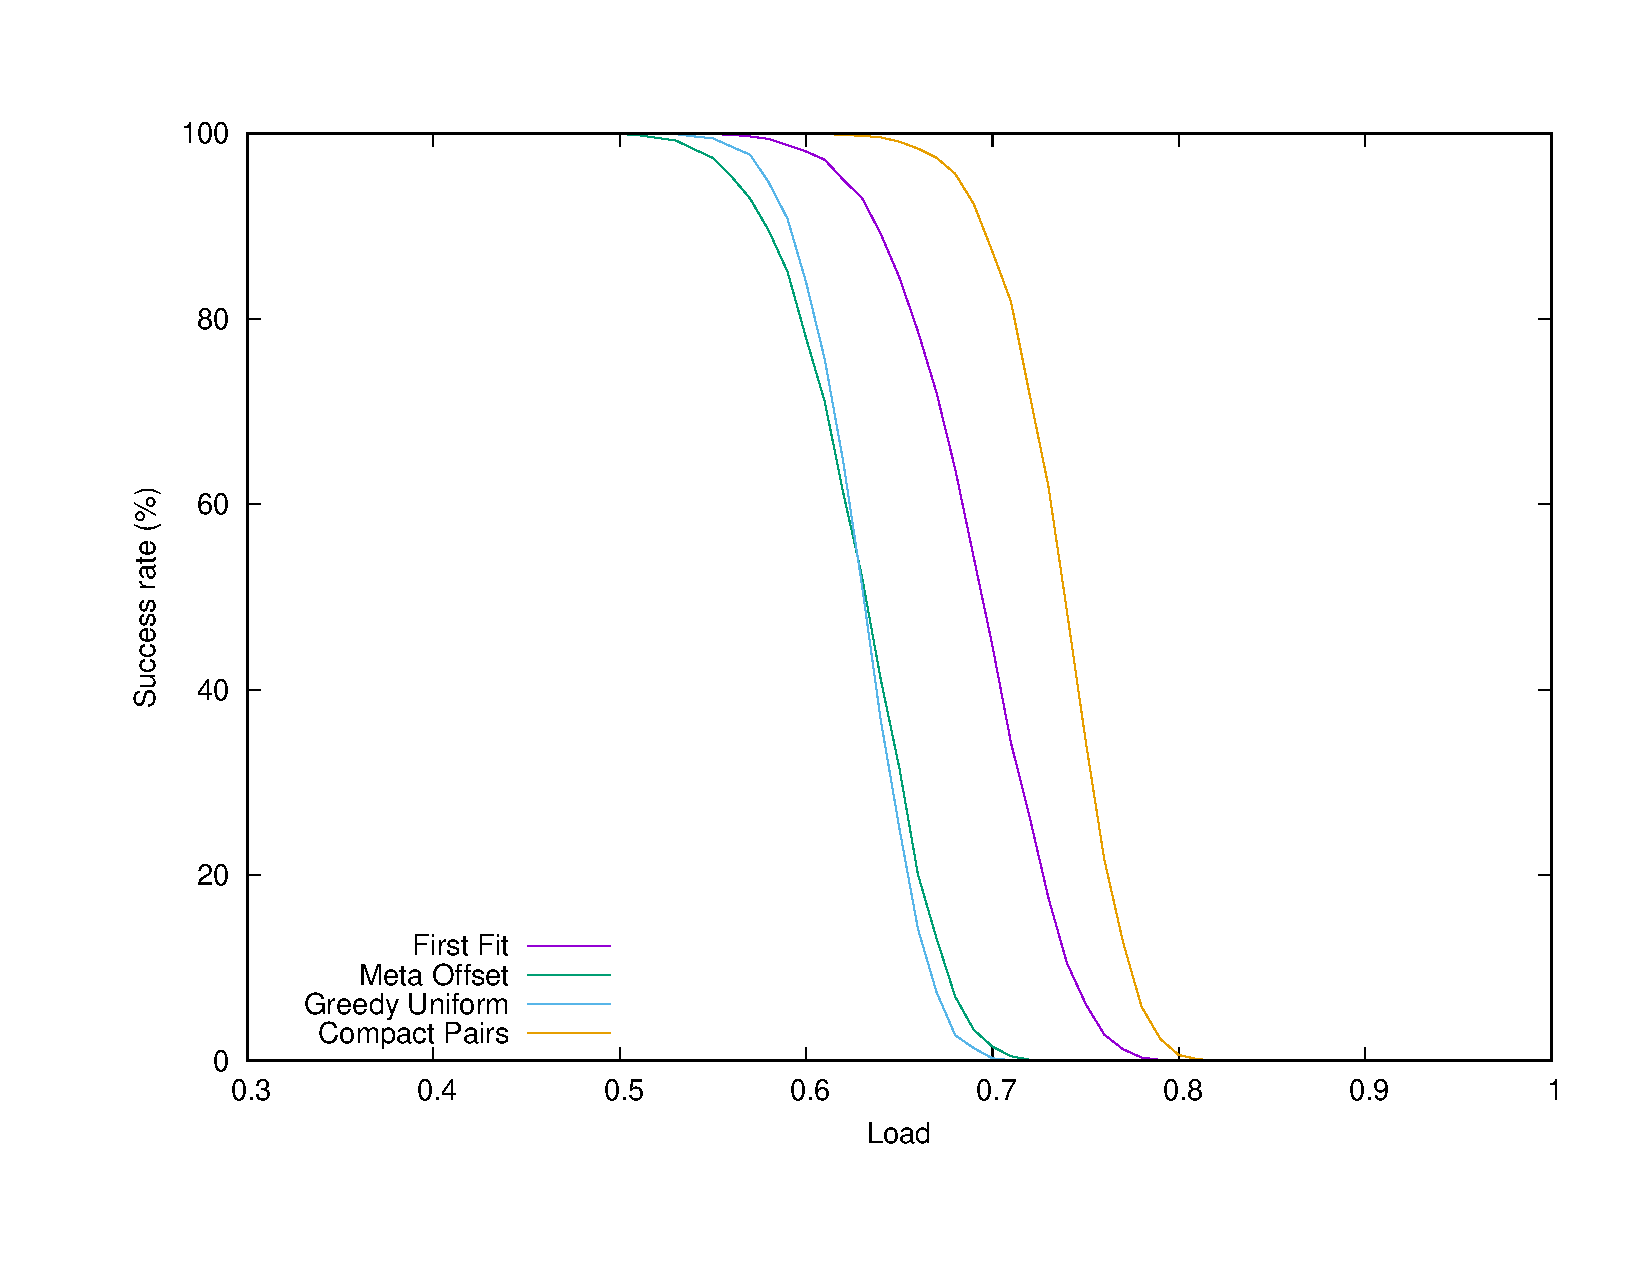
\includegraphics[scale=0.275]{Chapitre4PAZL/100messBig}

\captionof{figure}{Success rates of all algorithms for increasing loads, $\tau = 1000$, $P=100,000$}
\label{fig:100messBig}
\end{center} 
\end{minipage}
\begin{minipage}[c]{.45\linewidth}
\begin{center}  
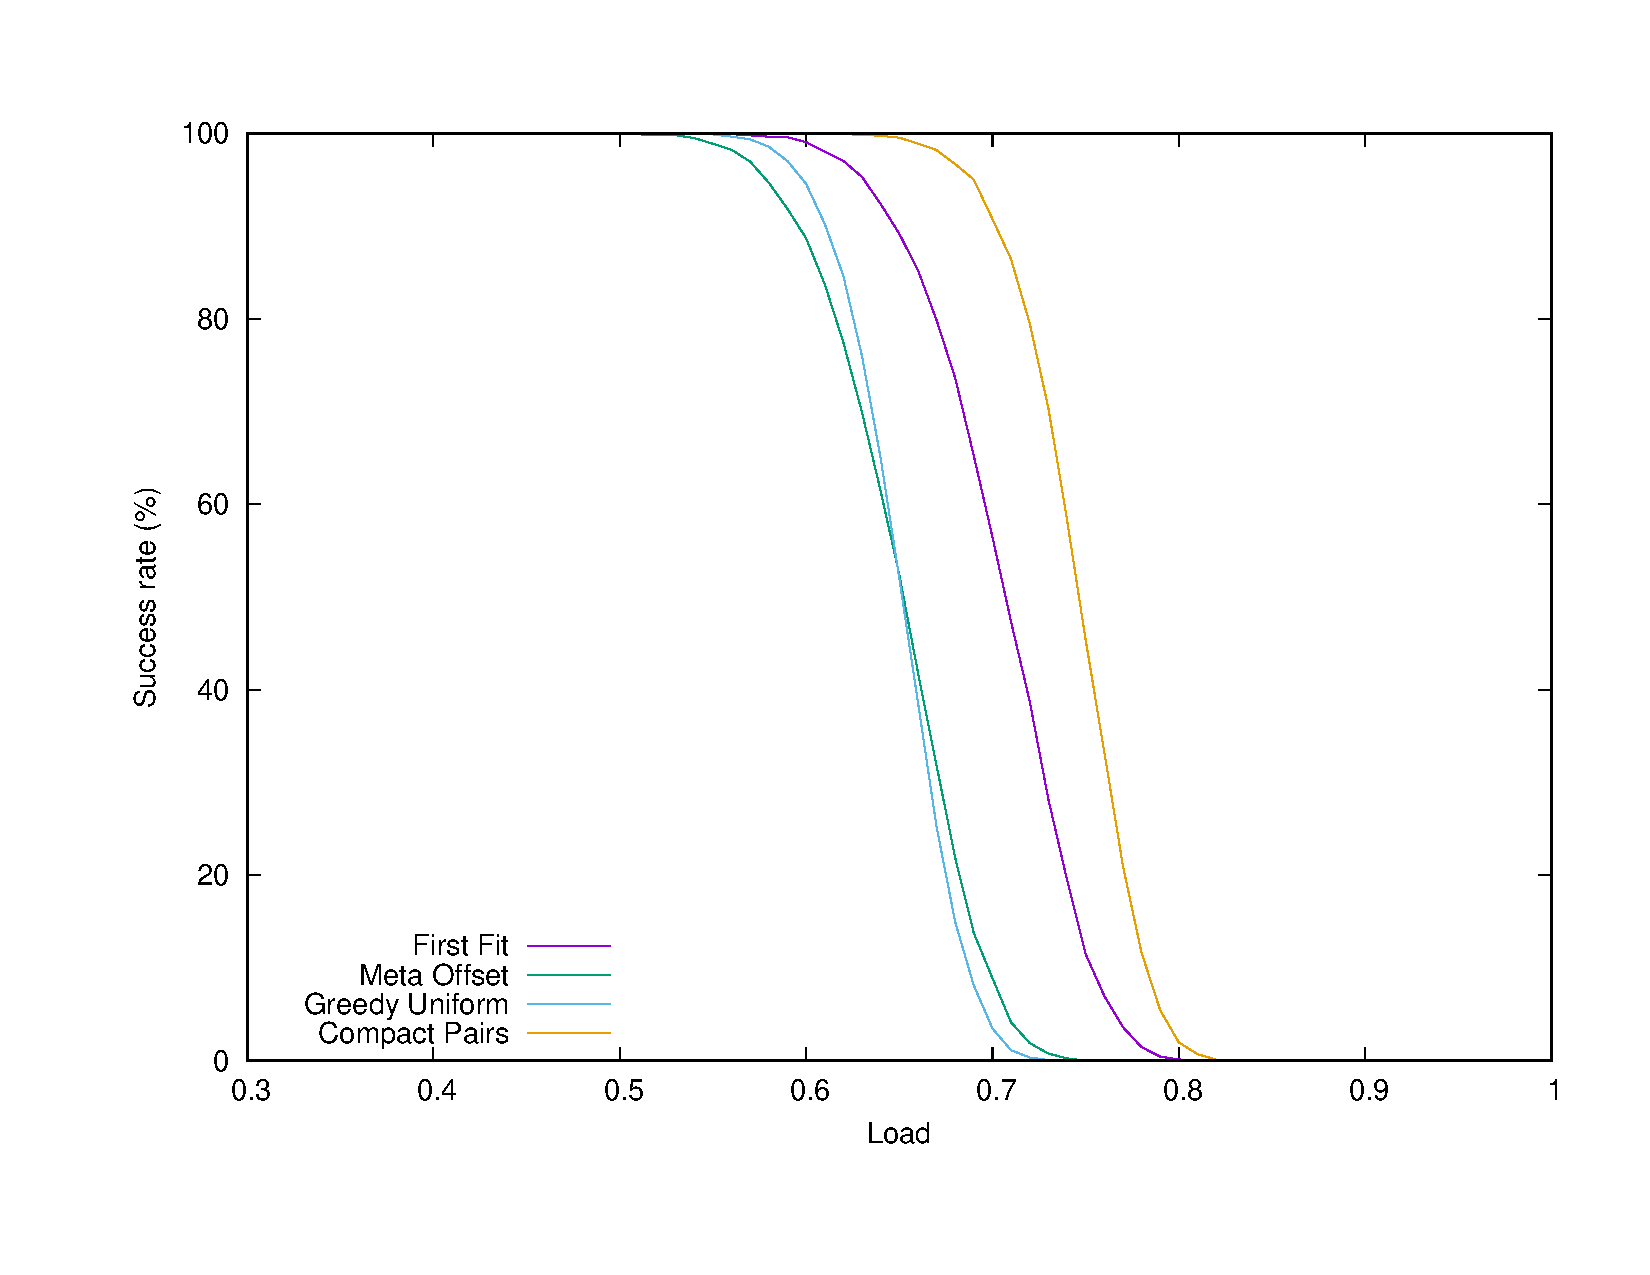
\includegraphics[scale=0.275]{Chapitre4PAZL/100messSmall}
\captionof{figure}{Success rates of all algorithms for increasing loads, $\tau = 10$, $P=1,000$}
\label{fig:100messSmall}
\end{center}
\end{minipage}



\begin{minipage}[c]{.49\linewidth}

\begin{center}
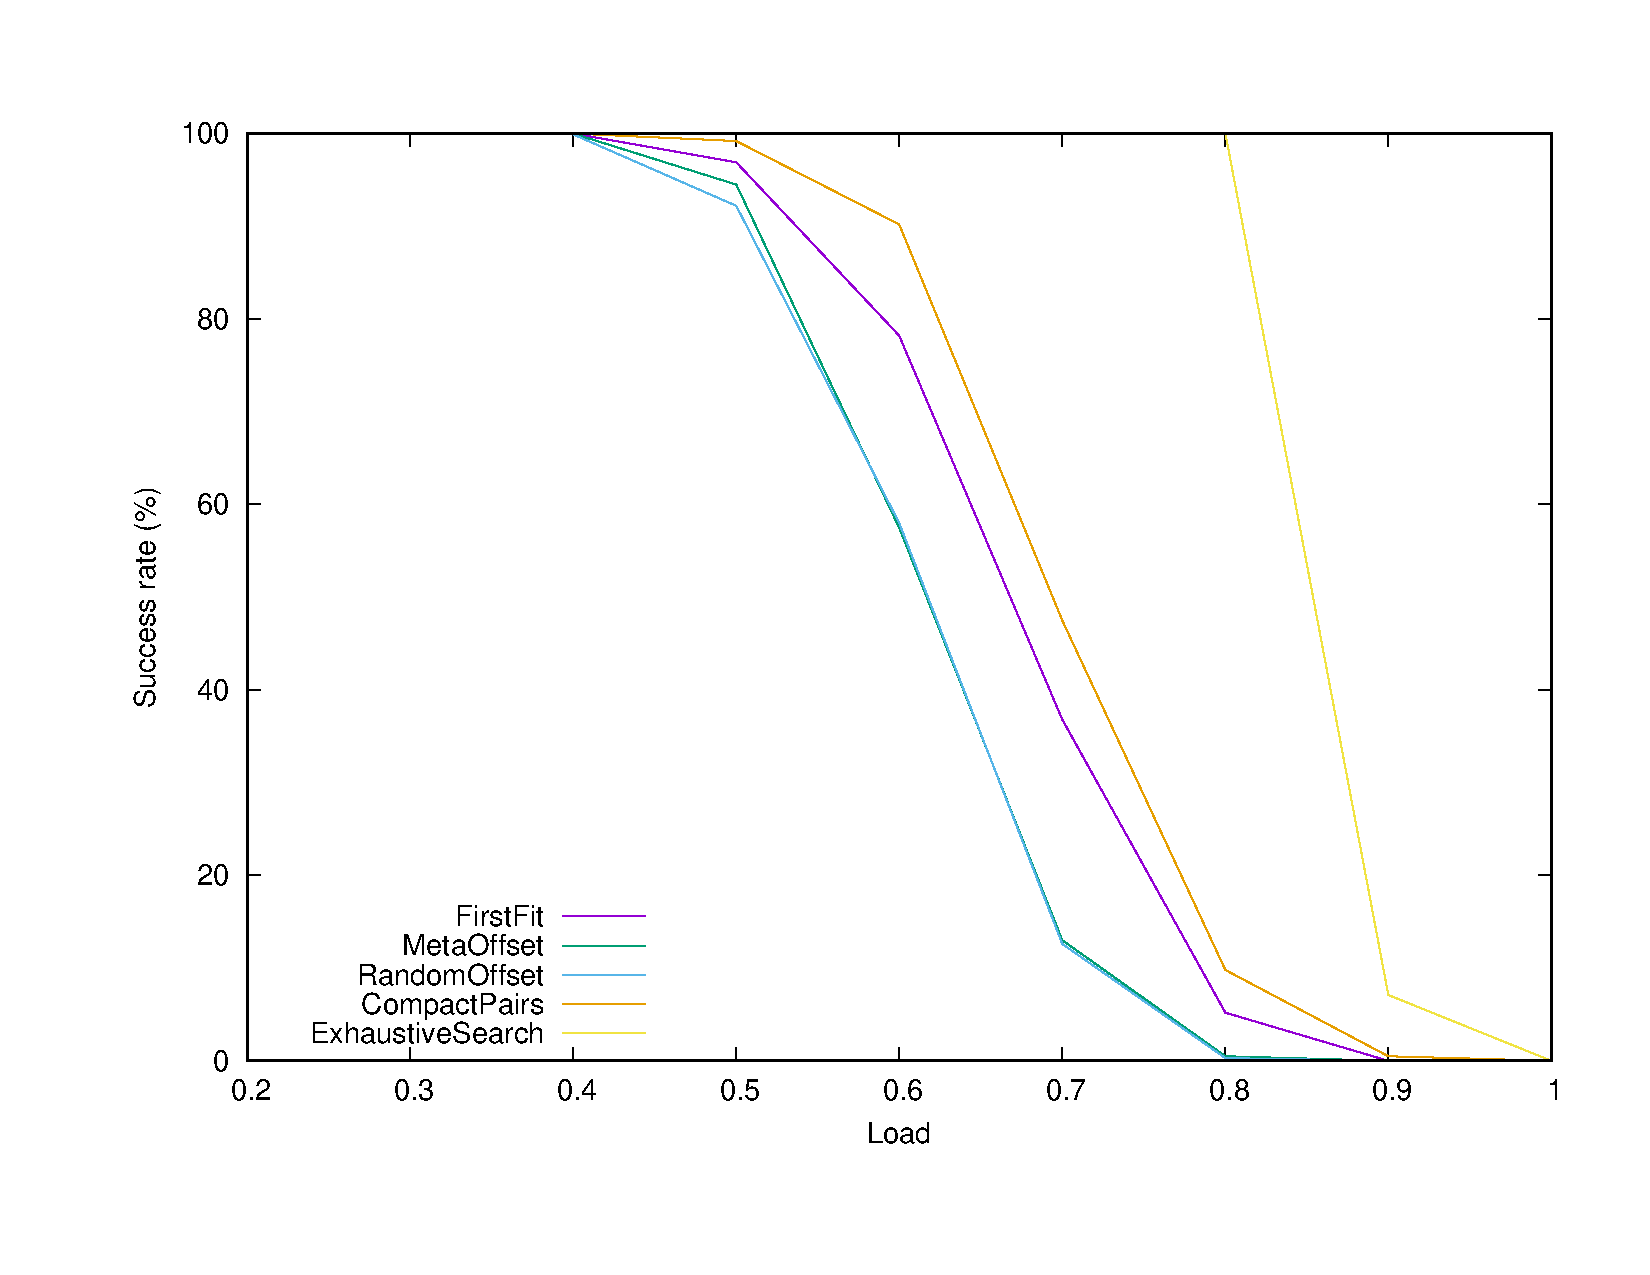
\includegraphics[scale=0.275]{Chapitre4PAZL/10mess}
\end{center}
\captionof{figure}{Success rates of all algorithms for increasing loads, $\tau = 1000$, $P=10,000$}
\label{fig:10mess}
\end{minipage}
\begin{minipage}[c]{.45\linewidth}
\begin{center}
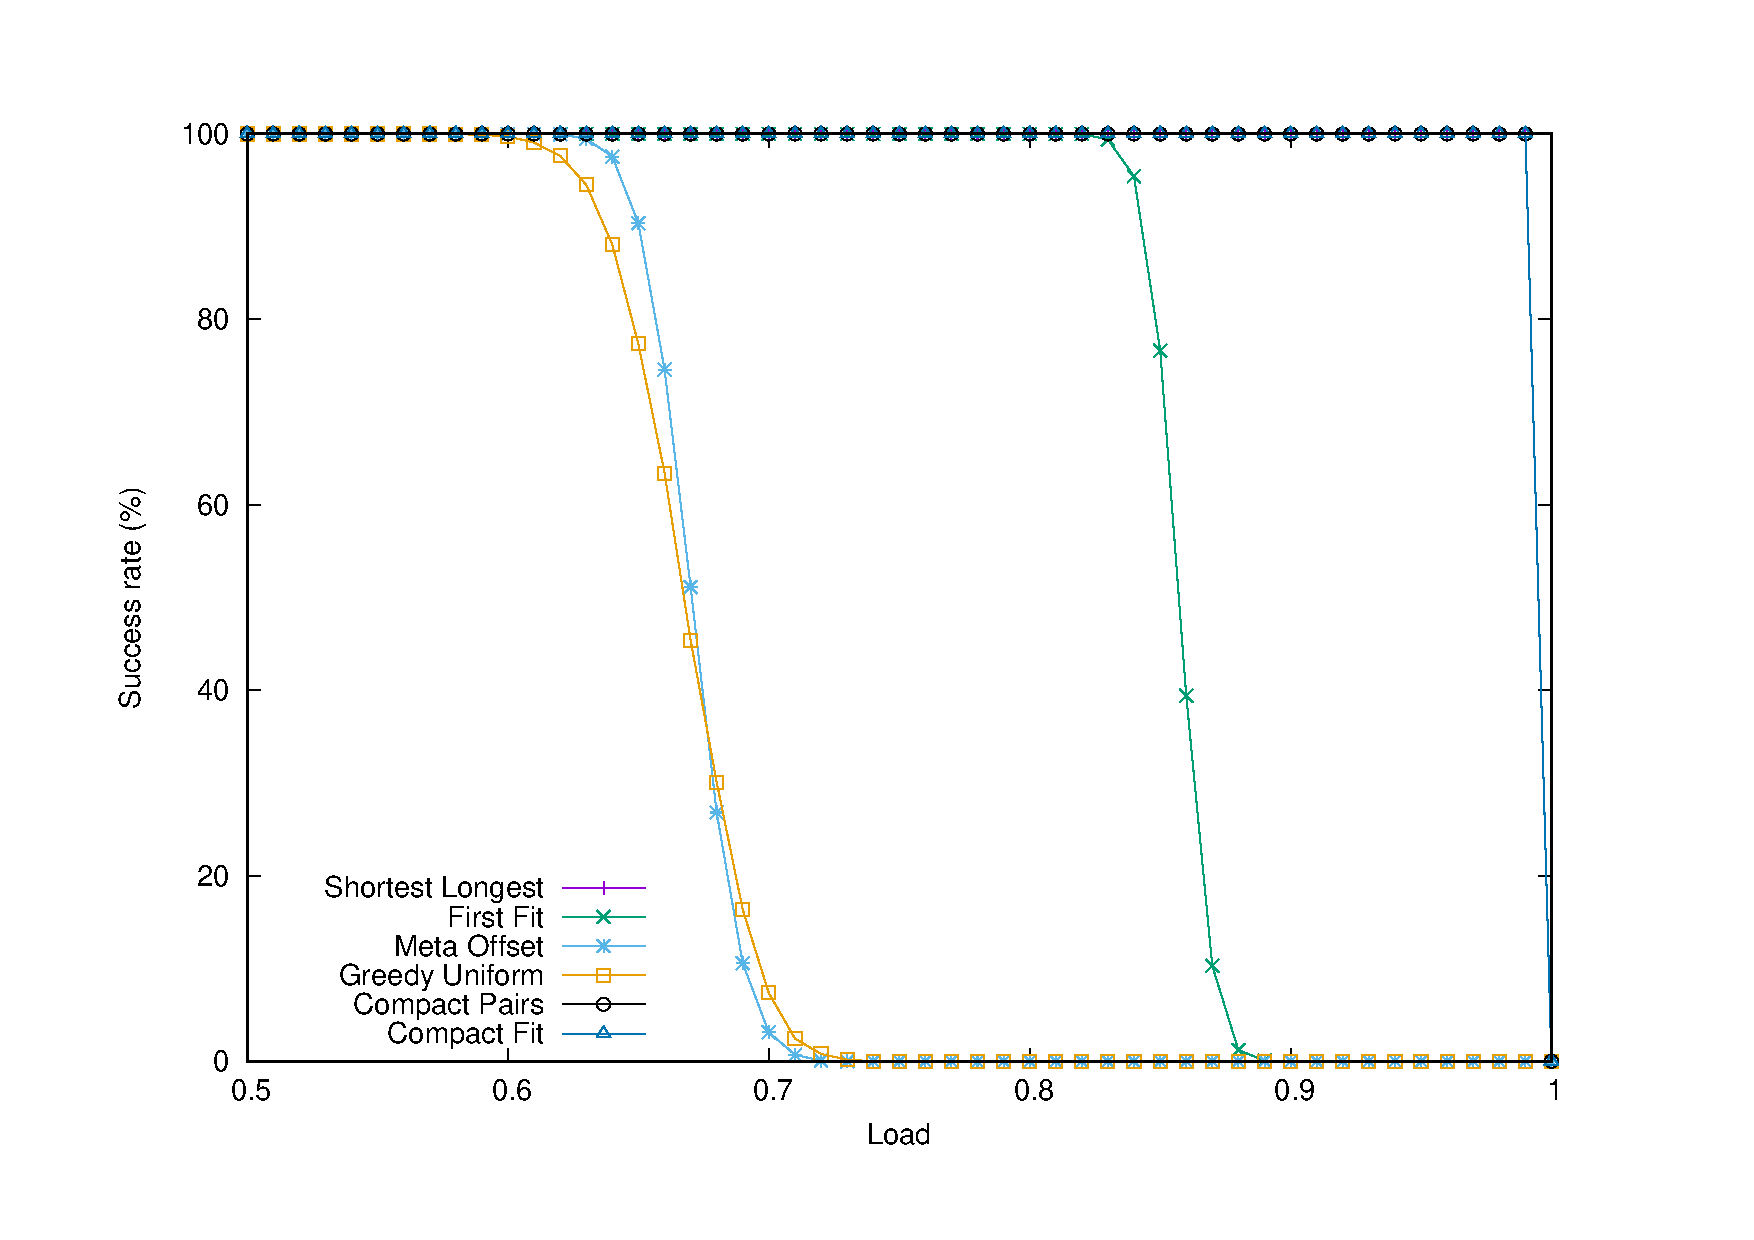
\includegraphics[scale=0.275]{Chapitre4PAZL/routestau}
\end{center}
\captionof{figure}{Same parameters as in Fig.~\ref{fig:100messBig}, delays uniformly drawn in $[\tau]$}
\label{fig:shortroutes}
\end{minipage}

\vspace{1cm}

In Figure~\ref{fig:100messBig} and Figure~\ref{fig:100messSmall} the performances of \shortestlongest are abysmal (falls to $10\%$ of success rate when the load is greater than $0.2$, and $0\%$ at $0.3$ of load) and are thus not represented in this figures, in order to focus on other algorithms. This can be explained by the fact it depends on the difference of size between the longest and the smallest route, which is large here since the delays are drawn in $[P]$. This observation is reinforced by the results of Figure~\ref{fig:10mess}. Indeed, since the number of route is lower than in the two previous experiment, the probability of drawing a set of delays with a large difference is lower, and thus the success rate of \shortestlongest is better. 

For all sets of parameters, the other greedy algorithms have the same relative performances. \metaoffset and \greedyuniform
perform the worst and have almost equal success rate. Remark that they have a $100\%$ success rate for load
less than $1/2$, while it is easy to build an instance of \pma of load $1/3 +\epsilon$ which makes them fail. 
The difference between the worst case analysis and the average case analysis is explained for \greedyuniform, when $\tau = 1$ in Section~\ref{sec:small}.

\firstfit performs better than \metaoffset while they have the same worst case. \compactpair, which is the best theoretically also performs well in the experiments, always finding assignments for load of $0.6$.  \compactfit, which is similar in spirit to \compactpair but is designed to have a good success rate on random instances is indeed better than  \compactpair, when there are enough datagrams.

As illustrated by Figure~\ref{fig:100messBig} and Figure~\ref{fig:100messSmall}, the size of the datagrams have little impact on the success rate of the algorithms, when the number of datagrams stay the same. Comparing Figure~\ref{fig:10mess} and Figure~\ref{fig:100messBig} shows that for more datagrams, the transition between success rate of $100\%$ to success rate of $0\%$ is faster.
Finally, the results of \ESCA in Figure~\ref{fig:10mess} show that the greedy algorithm are far from always finding a solution when it exists. Moreover, we have found an instance with load $0.8$ with no assignment, which gives an upper bound on the highest load for which \pma can always be solved positively.

We also investigate the behavior of the algorithms when the delay of the datagrams are drawn in $[\tau]$ in 
Figure~\ref{fig:shortroutes}. The difference from the case of large delay is that \compactpair and \compactfit are extremely efficient: they always find a solution for $99$ datagrams. It is expected, since all $\notationdelay'_i$ are equal in these settings and they will both build a $99$-compact tuples and thus can only fail for load $1$.


       As illustrated on Figure~\ref{fig:10mess}, when the load is larger than $0.5$, \ESCA finds more solutions than the greedy algorithms, which justifies its use. However, for load larger than $0.8$ there are instances for which there are no solutions to \pma. It means that with long routes and high load, looking for a bufferless assignment is far too restrictive. This justifies the design of algorithms for the general \pall problem, which we present in the next section. We will test them on $8$ long routes and a load between $1$ and $0.8$, parameters for which, as shown here, there are not always a bufferless assignment.
      
       The computation time of \ESCA is bounded by $O(4^nn!)$ as shown in Theorem~\ref{th:FPT}, but it can be much better in practice, either because it finds a solutions quickly or because a large part of the tree of compact assignments is pruned during the algorithm. We study the evolution of the running time  of the algorithm when $n$ grows in the following experiment. The weights of the arcs are drawn following a uniform distribution in $[P]$ and the load is set to $0.95$.  The table of Figure~\ref{fig:table} shows the time before the exhaustive search ends, for $8$ to $16$ routes, averaged on $100$ random star routed networks. This shows that for less than $20$ routes, which corresponds to all current topologies, the algorithm is efficient enough, but we should improve it further to work on more routes.
       
             \begin{figure}[h]
         \begin{center}
         \begin{tabularx}{0.9\textwidth}{|l|X|X|X|X|X|}
    \hline
   $n$ & $8$ & $10$& $12$&$14$& $16$\\
    \hline
   Time (s) & $6.10^{-5}$&$8.10^{-4}$&$2.10^{-2}$& $0.4$& $11$\\
    \hline
      \end{tabularx}
      \end{center}
      \caption{Running time of the exhaustive search.}
      \label{fig:table}
      \end{figure}



\section{Datagrams of Size One} \label{sec:small}

When $\tau = 1$ and the load is less than $1/2$, \emph{any greedy algorithm} solves \pma positively since $Fo(A) \leq (4\tau -2)|S| = 2|S|$ where $S$ is the number of scheduled datagrams. We give, in this section, a method which always finds an assignment for a load larger than $1/2$.

\subsection{Deterministic Algorithm}

To go above $1/2$ of load, we optimize a potential measuring how many offsets are available for all datagrams, scheduled or not. datagrams are scheduled while possible using any greedy algorithm. Then, when all unscheduled datagrams have no available offset, we use a Swap operation defined later, which improves the potential. When the potential is high enough, it ensures that there are two datagrams whose offset can be changed so that a new datagram can be scheduled. 

The algorithm is not greedy, since we allow to exchanging a scheduled datagram with an unscheduled one. It cannot work online, since it requires to know all delays of the datagrams in advance. 

\begin{definition}
The potential of a datagram of delay $\notationdelay$, for a partial assignment $A$
is the number of integers $i \in [P]$ such that $i$ is used in the first period and $i+\notationdelay \mod P$ is used in the second period.
\end{definition}

The computation of the potential of a datagram of delay $3$, is illustrated in Fig.~\ref{fig:datagrampotential}.
The potential of a datagram counts the configurations which reduce the number of forbidden offsets.
Indeed, when $i$ is used in the first period and $i+\notationdelay \mod P$ is used in the second period,
then the same offset is forbidden \emph{twice} for a datagram of delay $\notationdelay$. Hence, the potential of a datagram is related to the number of possible offsets as stated in the following lemma. 
\begin{figure}
 \begin{center}
\includegraphics[scale=1]{Chapitre4PAZL/messagepotential}
\end{center}
\caption{A datagram of delay $3$ has potential $2$ in the represented assignment}
\label{fig:datagrampotential}
\end{figure} 

\begin{lemma}
Given a partial assignment $A$ of size $s$, and $i$ an unscheduled datagram of potential 
$v$, then the set $\{o \mid A(i \rightarrow o) \text{ has no collision}\}$ is of size $P - 2s + v$.
\end{lemma}

For our algorithm, we need a global measure of quality of a partial assignment, 
that we try to increase when the algorithm fail to schedule new datagrams. 
We call our measure \textbf{the potential of an assignment} and we denote it by $Pot(A)$, it is the sum of potentials of all datagrams in the instance.


\begin{definition}
The potential of a position $i$, for a partial assignment $A$, is the number of datagrams of delay $\notationdelay$ such that $i+\notationdelay \mod P$ is used by a datagram scheduled by $A$. 
\end{definition}

\begin{figure}
 \begin{center}
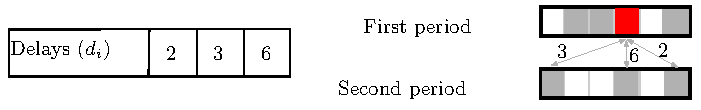
\includegraphics[scale=1]{Chapitre4PAZL/positionspotential}
\end{center}
\caption{Shaded position potential $2$, in this assignment}
\label{fig:positionpotential} 
\end{figure}

The potential of a position is illustrated in Figure~\ref{fig:positionpotential}.
Instead of decomposing the global potential as a sum over datagrams, it can be understood
as a sum over positions, as stated in the next lemma.

\begin{lemma}\label{lemma:pot_pos}
The sum of potentials of all positions used in the first period by datagrams scheduled by $A$ is equal to $Pot(A)$.  
\end{lemma}

By definition of the potential of a position, we obtain the following simple invariant.

\begin{lemma}\label{lemma:inv}
The sum of potentials of all positions for a partial assignment with $k$ scheduled datagrams is $nk$.  
\end{lemma}

 As a consequence of this lemma, $Pot(A) \leq nk$. Let us define a \textbf{Swap operation},
 which guarantees to obtain at last half the maximal value of the potential.
Let $A$ be some partial assignment of size $s$ and let $i$ be an unscheduled datagram of delay $\notationdelay$. 
Assume that $i$ cannot be used to extend $A$. The Swap operation is the following: 
select a free position $o$ in the first period, remove the datagram which uses the position $o+\notationdelay$ in the second period from $A$ and extend $A$ by $i$ with offset $o$. We denote this operation by $Swap(i,o,A)$.

\begin{lemma}\label{lemma:swap}
Let $A$ be some partial assignment of size $k$ and let $i$ be an unscheduled datagram. If $i$ cannot be used to extend $A$, then either $Pot(A) \geq kn/2$ or there is an $o$ such that $Pot(Swap(i,o,A)) > Pot(A)$.
\end{lemma}

\begin{proof}
The positions in the first period can be partitioned into $P_{u}$ the positions used by some scheduled datagram and $P_{f}$ the positions unused.
Let $V_f$ be the sum of the potentials of the positions in $P_f$ and let $V_u$ be the sum of the potentials of the positions in $P_u$. By Lemma~\ref{lemma:inv}, since $P_f$ and $P_u$ partition the positions, we have $V_f + V_u = kn$. Moreover, by Lemma~\ref{lemma:pot_pos}, $Pot(A) = V_u$, then $V_f + Pot(A) = kn$.

By hypothesis, $i$ cannot be scheduled, then, for all $p \in P_{f}$, $p+\notationdelay_i$ is used in the second period. Let us define the function $F$ which associates to $p \in P_{f}$ the position $A(j)$ such that there is a scheduled datagram $j$ which uses $p+d$ in the second period, that is $A(j) + \notationdelay_j = p + d \mod P$. The function $F$ is an injection from $P_{f}$ to $P_u$. Remark now that, if we compare $Swap(i,p,A)$ to $A$, on the second period the same positions are used. Hence, the potential of each position stay the same after the swap. As a consequence, doing the operation $Swap(i,p,A)$ adds to $Pot(A)$ the potential of the position $p$ and removes the potential of the position $F(p)$. 

Assume now, to prove our lemma, that for all $p$, $Pot(Swap(i,p,A)) \leq Pot(A)$. It implies that for all $p$, the potential of $p$ is smaller than the potential of $F(p)$. Since $F$ is an injection from $P_f$ to $P_u$, we have that $V_f \leq V_u = Pot(A)$. Since $V_f + Pot(A) = kn$, we have that $Pot(A) \geq kn/2$.
\end{proof}

Let us precisely describe the algorithm \swapandmove:  datagrams are scheduled while possible by \firstfit and then the Swap operation is applied while it increases the potential. When the potential is maximal, \swapandmove schedule a new datagram by moving at most two scheduled datagrams to other available offsets. If it fails to do so, \swapandmove stops, otherwise the whole procedure is repeated. We analyze \swapandmove in the following theorem.

\begin{theorem}
\swapandmove solves positively \pma, in polynomial time, for instances with $\tau =1$ and load less than $1/2 + (\sqrt{5}/2 -1) \approx 0,618$.
\end{theorem}

\begin{proof}
We determine for which value of the load \swapandmove always works. We let $n = (1/2 + \epsilon)P$ be the number of datagrams, the load is $1/2 + \epsilon$. We need only to study the case when $n-1$ datagrams are scheduled by $A$ and \swapandmove tries to schedule the last one, since the previous steps are similar but easier. 

Let $\notationdelay$ be the delay of the unscheduled datagram. We consider the pairs 
of times $(o,o+d)$ for $o \in [P]$. Since the datagram
cannot be scheduled, there are three cases. First, $o$ is unused in the first period but $o+d$ is used in the second period. Since there are $n-1$ scheduled datagrams, there are $P-n+1$ such value of $o$. If a datagram using the time $o+d$ in the second period can be scheduled elsewhere, so that the unscheduled datagram can use offset $o$, then \swapandmove succeeds.
Otherwise, the datagram has no possible offsets, which means its potential is equal to $2(\epsilon P -1)$.
The second case is symmetric: $o$ is used in the first period but $o+d$ is unused in the second period. 
Finally, we have the case $o$ is used in the first period and $o+d$ is used in the second period.  There are $2(\epsilon P -1)$ such values of $o$. If the two datagrams using times 
$o$ and $o+d$ can be rescheduled so that offset $o$ can be used for the unscheduled datagram,
then \swapandmove succeeds. This is always possible when one datagram is of potential at least $2\epsilon P -1$ and the other of potential at least $2\epsilon P + 1$. Since the datagrams must be of potential more than $2(\epsilon P -1)$ and at most $n-1$, it is satisfied when the sum of the two potentials is at least $2(\epsilon P -1) + n$.

If we assume that \swapandmove was unable to schedule the last datagram by moving two scheduled datagrams, the previous analysis gives us a bound on twice $Pot(A)$: 
$$ 2Pot(A) \leq 2(P-n+1) 2(\epsilon P -1) + 2(\epsilon P -1)(2(\epsilon P -1) + n) $$
$$ Pot(A) \leq (\epsilon P -1) (P + n)$$
By Lemma~\ref{lemma:swap}, we know that $Pot(A) \geq n(n-1)/2$, hence 
\swapandmove must succeed when
$$n(n-1)/2 \geq  (\epsilon P -1) (P + n).$$
By expanding and simplifying, we obtain a second degree inequation in $\epsilon$, $1/4 - 2\epsilon - \epsilon ^2 \geq  0$.
Solving this inequation yields $\epsilon \leq \sqrt{5}/2 -1$.


Let us prove that \swapandmove is in polynomial time. All Swap operations 
strictly increase the potential. Moreover, when one or two datagrams are moved, the potential may decrease but
a datagram is added to the partial assignment. The potential is bounded by $O(n^2)$ and the move operations all together can only remove $O(n^2)$ to the potential, hence there are at most $O(n^2)$ Swap operations during \swapandmove. A Swap operation can be performed in time $O(n)$, since for a given datagram, all free offsets must be tested and the potential is evaluated in time $O(1)$ (by maintaining the potential of each position). This proves that Swap and Move is in $O(n^3)$.  
\end{proof}

Consider a partial assignment of size $n' = (1/2 + \epsilon)P$, and a datagram of delay $\notationdelay$.
If we consider all $n'$ used offsets $o$ and all times time $o+d$ in the second period, 
then $o$ and $o+d$ are both used for at least $n' - (P -n') = 2\epsilon P$ values of $o$.
The potential of any datagram is thus larger or equal to $2\epsilon P$. When a datagram cannot be scheduled, its potential is less or equal to $2\epsilon P$, hence it is equal to $2\epsilon P$.

Hence, the potential of any assignment of size $n'$ is at least $2\epsilon P n $. As a consequence, the method of Lemma~\ref{lemma:swap} will guarantee a non-trivial potential for $2\epsilon P n <  nn'/2$, that is $\epsilon < 1/6$. Any algorithm relying on the potential and the Swap operation cannot be guaranteed to work for load larger than $2/3 = 1/2 + 1/6$. However, we may hope to improve on the analysis of Lemma~\ref{lemma:swap}, since it is not optimal: $2\epsilon P$ positions in $P_{u}$ are not taken into account in the proof. 

We conjecture that \swapandmove works for load up to $2/3$. 
On random instances, we expect the potential to be higher than the stated bound and to be better spread on the datagrams, which would make \swapandmove works for larger loads, as it is indeed observed in experiments (see Section~\ref{sec:perf_small}).

\subsection{Randomized Algorithm for Random Instances}

We would like to understand better the behavior of our algorithms
on instances drawn uniformly at random. To this aim, we analyze the algorithm \greedyuniform, defined as follows: for each datagram in the order of the input, choose one of the offsets, which does not create a collision with the current partial assignment, uniformly at random. 

We analyze \greedyuniform over random instances:  all datagrams have 
their delays drawn independently and uniformly in $[m]$. We compute the probability of success of \greedyuniform over all random choices by the algorithm \emph{and all possible instances}. 
It turns out that this probability, for a fixed load strictly less than one, goes to one when $m$ grows. 
For a given partial assignment, we are only interested in its \textbf{trace}: the set of times which are used in the first and second period. Hence, if $n$ datagrams are scheduled in a period of size $m$, the trace of an assignment is a pair of subsets of $[m]$ of size $n$. We now show that these traces are produced uniformly by \greedyuniform.

\begin{theorem}
The distribution of traces of assignments produced by \greedyuniform when it succeeds, from instances drawn uniformly at random, is also uniform.
\end{theorem}
\begin{proof}
The proof is by induction on $n$, the number of datagrams. It is clear for $n=1$,
since the delay of the first datagram is uniformly drawn and all offsets can be used.
Assume now the theorem true for some $n>1$. \greedyuniform, by induction hypothesis has produced
uniform traces from the first $n$ datagrams.  Hence, we should prove that, if we draw delays
of the $n+1^{th}$ datagram randomly, extending the trace by a random possible offset produces a random distribution on the traces of size $n+1$. 

 If we draw an offset uniformly at random (among all $m$ offsets) and then extend the trace by scheduling the last datagram at this offset or fail, the distribution over the traces of size $n+1$ is the same as what produces \greedyuniform. Indeed, all offsets which can be used to extend the trace have the same probability to be drawn. Since all delays are drawn independently, we can assume that, given a trace, we first draw an offset uniformly, then draw uniformly the delay of the added datagram and add it to the trace if it is possible. This proves that all extensions of a given trace are equiprobable. Thus, all traces of size $n+1$ are equiprobable, since they each can be formed from $(n+1)^2$ traces of size $n$ by removing one used time from the first and second period. This proves the induction and the theorem.
\end{proof}

Since \greedyuniform can be seen as a simple random process on traces by Th.~\ref{theorem:uniform}, it is easy to analyze its probability of success.

\begin{theorem}\label{theorem:uniform}
The probability over all instances with $n$ datagrams and period $m$ that \greedyuniform solves $\pma$ positively is $$\displaystyle{\prod_{i=m/2}^{n-1}(1 - \frac{\binom{n}{2i-m}}{\binom{m}{i}})}.$$
\end{theorem}
\begin{proof}
We evaluate $\Pr(m,n)$ the probability that \greedyuniform fails at the $n^{th}$ step assuming it has not failed before. It is independent of the delay of the $n^{th}$ datagram. Indeed, the operation which adds one to all times used 
in the second period is a bijection on the set of traces of size $n-1$. It is equivalent to remove one to the delay of the $n^{th}$ datagram. We can thus assume that the delay is zero.

Let $S_1$ be the set of times used in the first period by the $n-1$ first datagrams
and $S_2$ the set of times used in the second period. We can assume that $S_1$ is fixed, since all subsets of the first period are equiprobable and because $S_2$ is independent of $S_1$ (Th.~\ref{theorem:uniform}). There is no possible offset for the $n^{th}$ datagram, if and only if $S_1 \cup S_2 = [m]$. It means that $S_2$ has been drawn such that it contains $[m] \setminus S_1$. By Th.\ref{theorem:uniform}, $S_2$ is uniformly distributed over all sets of size $n-1$. Hence, the probability that  $[m]  \setminus S_1 \subseteq S_2$  is the probability to draw a set of size $n-1$ which contains $m-n + 1$ fixed elements. This proves $\Pr(m,n) = \frac{\binom{n}{2(n-1)-m}}{\binom{m}{n-1}}$.

From the previous expression, we can derive the probability of success of \greedyuniform by a simple product of 
the probabilities of success $(1 - \Pr(m,i))$ at step $i$, for all $i \leq n$, which proves the theorem. 
\end{proof}


If we fix the load $\lambda = n/m$, we can bound $P(m,n)$ using Stirling formula. We obtain for some constant $C$, 
that $P(m,n) \leq C \left(\frac{\lambda^{2\lambda}}{(2\lambda -1)^{2\lambda -1}}\right)^m$.
We let $f(\lambda) = \frac{\lambda^{2\lambda}}{(2\lambda -1)^{2\lambda -1}}$.
The derivative of $f$ is strictly positive for $1/2 < \lambda < 1$ and $f(1) = 1$, hence 
$f(\lambda) < 1$ when $\lambda < 1$. By a simple union bound, the probability that \greedyuniform fails is bounded 
by $C \lambda m f(\lambda)^m$, whose limit is zero when $m$ goes to infinity. 
It explains why \greedyuniform is good in practice for large $m$. 




\subsection{Experimental Results} \label{sec:perf_small}


In this section, the performance on random instances of the algorithms presented in Sec.~\ref{sec:small} is experimentally characterized. The settings are as in Section~\ref{sec:perf_large}, with $\tau = 1$.
Because $\tau =1$, the algorithms based on meta-offsets are not relevant anymore. The evaluated algorithms are:


\begin{itemize}
  \item \firstfit
  \item \greedyuniform 
  \item \greedypotential, a greedy algorithm which leverages the notion of potential introduced for Swap. 
  It schedules the datagrams in arbitrary order, choosing the possible offset which maximizes the potential of the unscheduled datagrams
  \item \swapandmove 
  \item \ESCA
\end{itemize}

In Figure~\ref{fig:tau1}, the performances of \shortestlongest are the same as in Figure~\ref{fig:100messBig} and Figure~\ref{fig:100messSmall}( $10\%$ for load  $0.2$, and $0\%$ at $0.3$ of load). The algorithm seems to performs better on Figure~\ref{fig:tau1-10mess} ($25\%$ of success at load $0.5$), but the algorithm is not interesting since \greedypotential, \firstfit or \greedyuniform have much better success rate for a similar complexity.

For the other algorithms, as in Section~\ref{sec:perf_large}, the success rate on random instances is much better than the bound given by worst case analysis. In the experiment presented in Figure~\ref{fig:tau1}, all algorithms succeed on all instances when the load is less than $0.64$. \greedyuniform behaves exactly as proved in Theorem~\ref{theorem:uniform}, with a very small variance. The performance of \swapandmove and of its simpler variant \greedypotential, which optimizes the potential in a greedy way, are much better than \firstfit or \greedyuniform. Amazingly, \swapandmove always finds an assignment when the load is less than $0.95$. \swapandmove is extremely close to \ESCA, but for $P=10$ and load $0.9$ or $1$, it fails to find some assignments, as shown in Figure.~\ref{fig:tau1-10mess}.

\begin{minipage}[c]{.49\linewidth} 
\begin{center} 
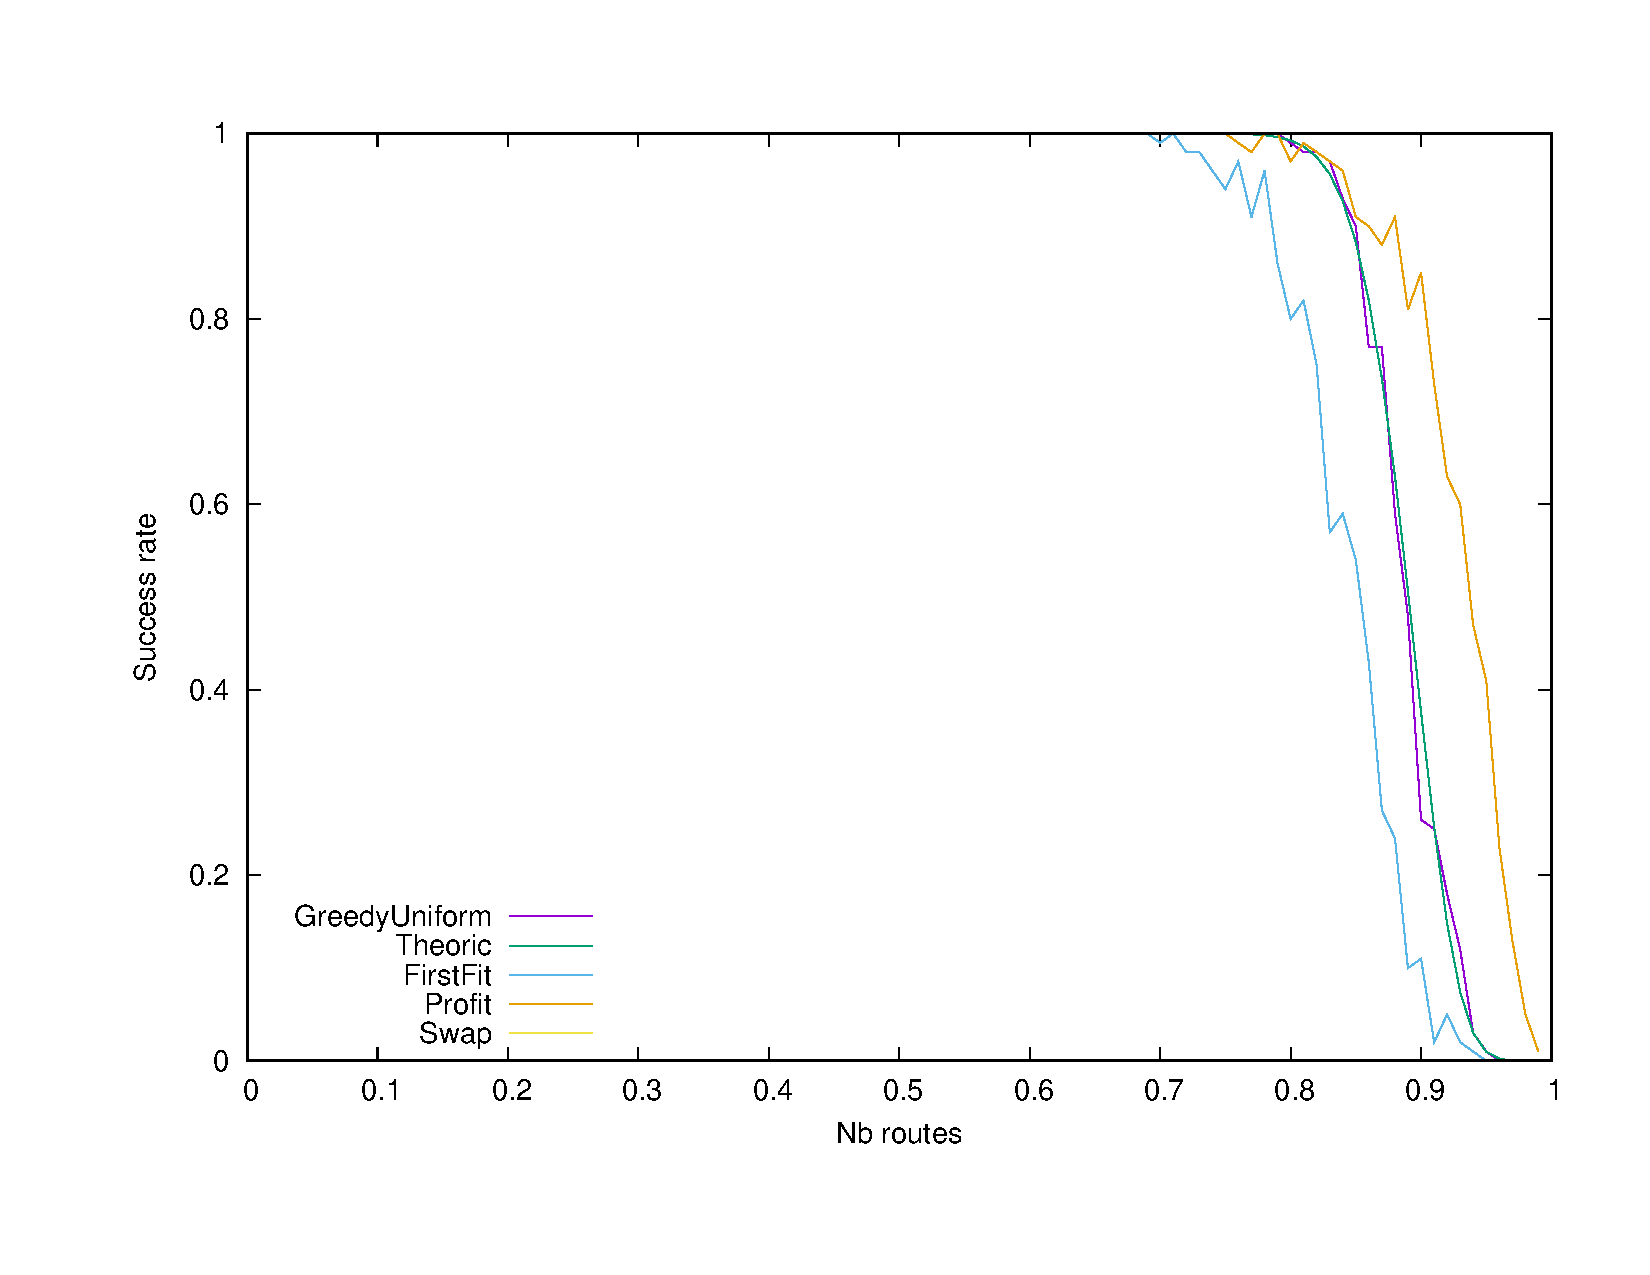
\includegraphics[scale=0.275]{Chapitre4PAZL/success_tau1} 
\end{center}
\captionof{figure}{Success rates of all algorithms for increasing loads, $\tau = 1$ and $P=100$}
\label{fig:tau1}
\end{minipage}
\begin{minipage}[c]{.45\linewidth} 

\begin{center}
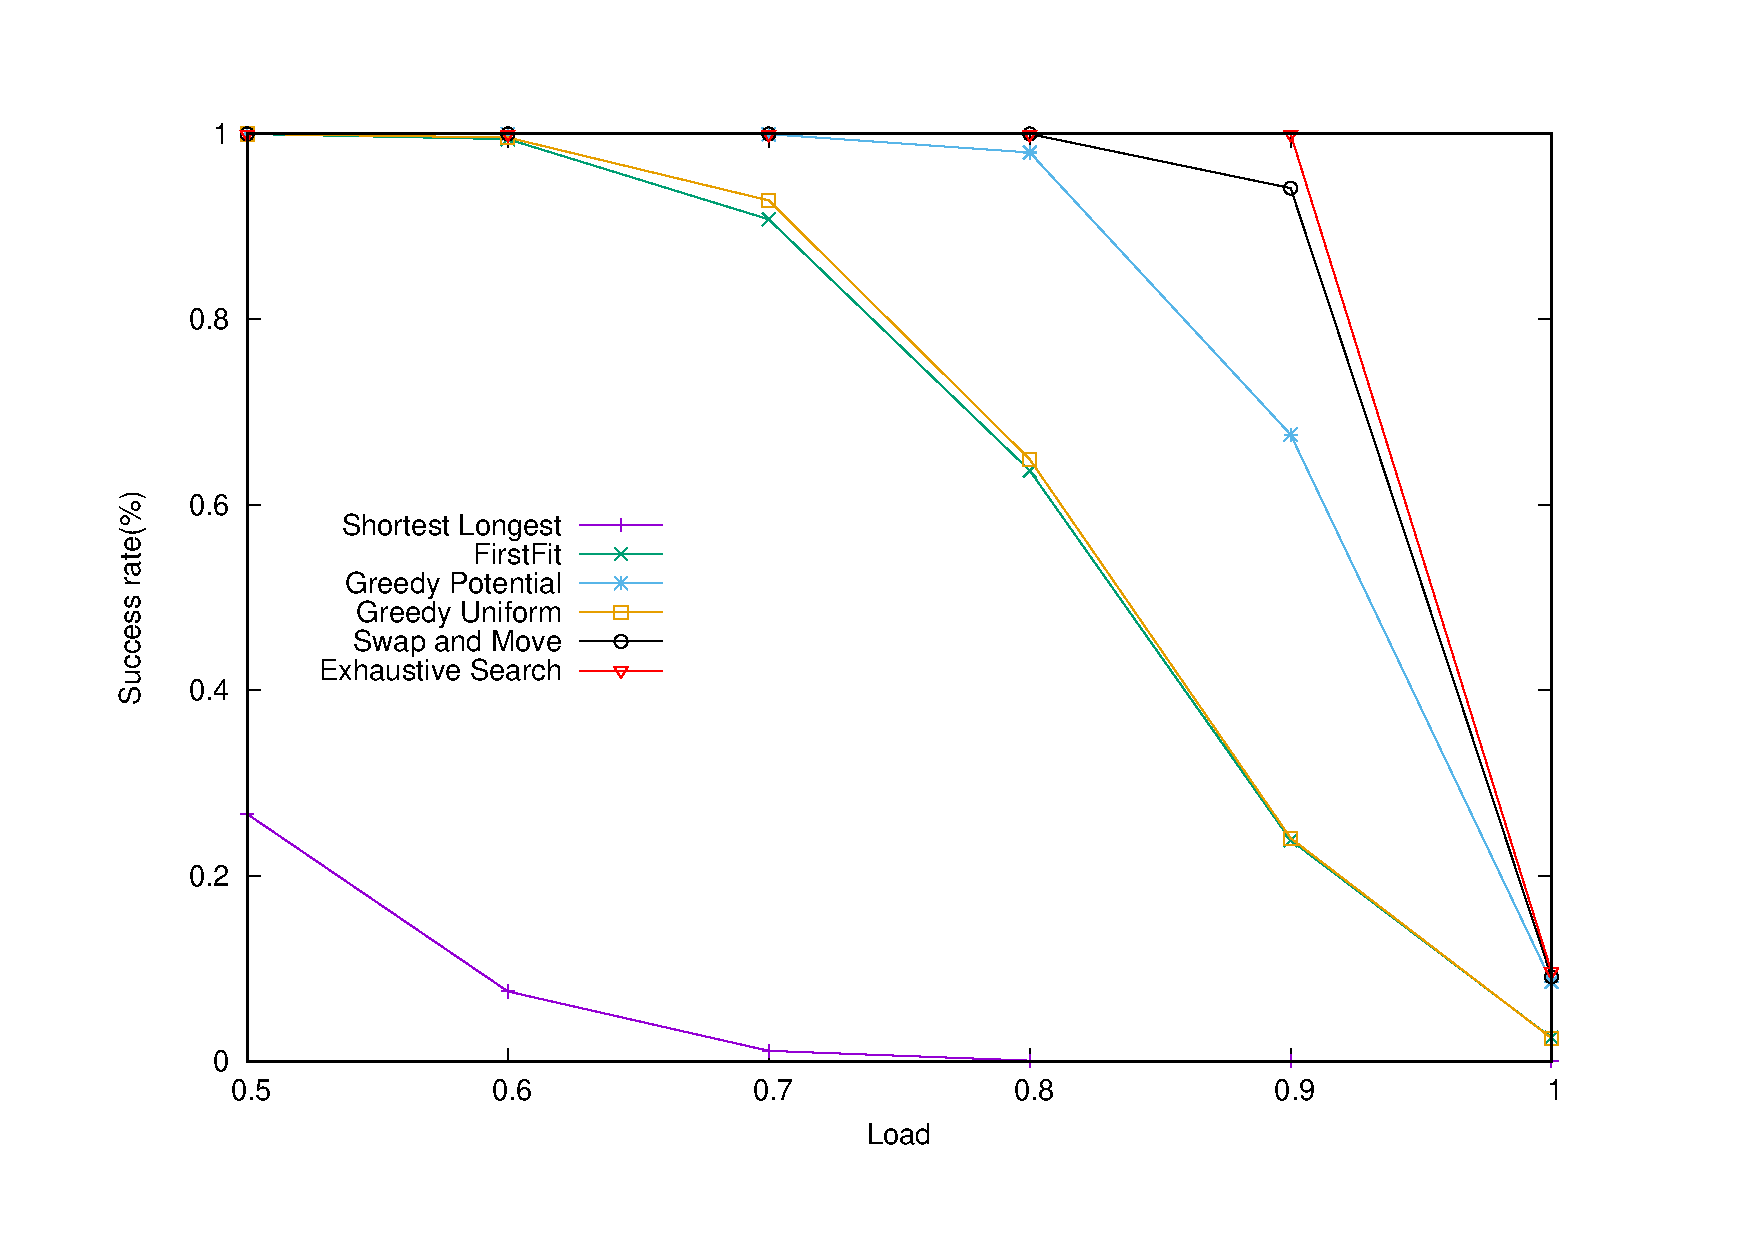
\includegraphics[scale=0.275]{Chapitre4PAZL/tau110}
\end{center}
\captionof{figure}{Success rates of all algorithms for increasing loads, $\tau = 1$ and $P=10$}
\label{fig:tau1-10mess}
\end{minipage}
 \vspace{1cm}

 Finally, we evaluate the computation times of the algorithms to understand whether they scale to large instances. We present the computation times in Fig.~\ref{fig:timelog} and we choose to consider instances of load $1$, since they require the most computation time for a given size. The empirical complexity of an algorithm is evaluated by a
 linear regression on the function which associates to $\log(n)$, the log of the computation time of the algorithm on $n$ datagrams.  \firstfit, \greedyuniform, \shortestlongest and \swapandmove scale almost in the same way, with an empirical complexity slightly below $O(n^2)$, while \greedypotential has an empirical complexity of $O(n^3)$. The empirical complexity corresponds to the worst case complexity we have proved, except for \swapandmove which is in $O(n^3)$ worst case. There are two explanations: most of the datagrams are scheduled by the fast \firstfit subroutine and most Swap operations improve the potential by more than $1$, as we assume in the worst case analysis.

\begin{figure}
 \begin{center}
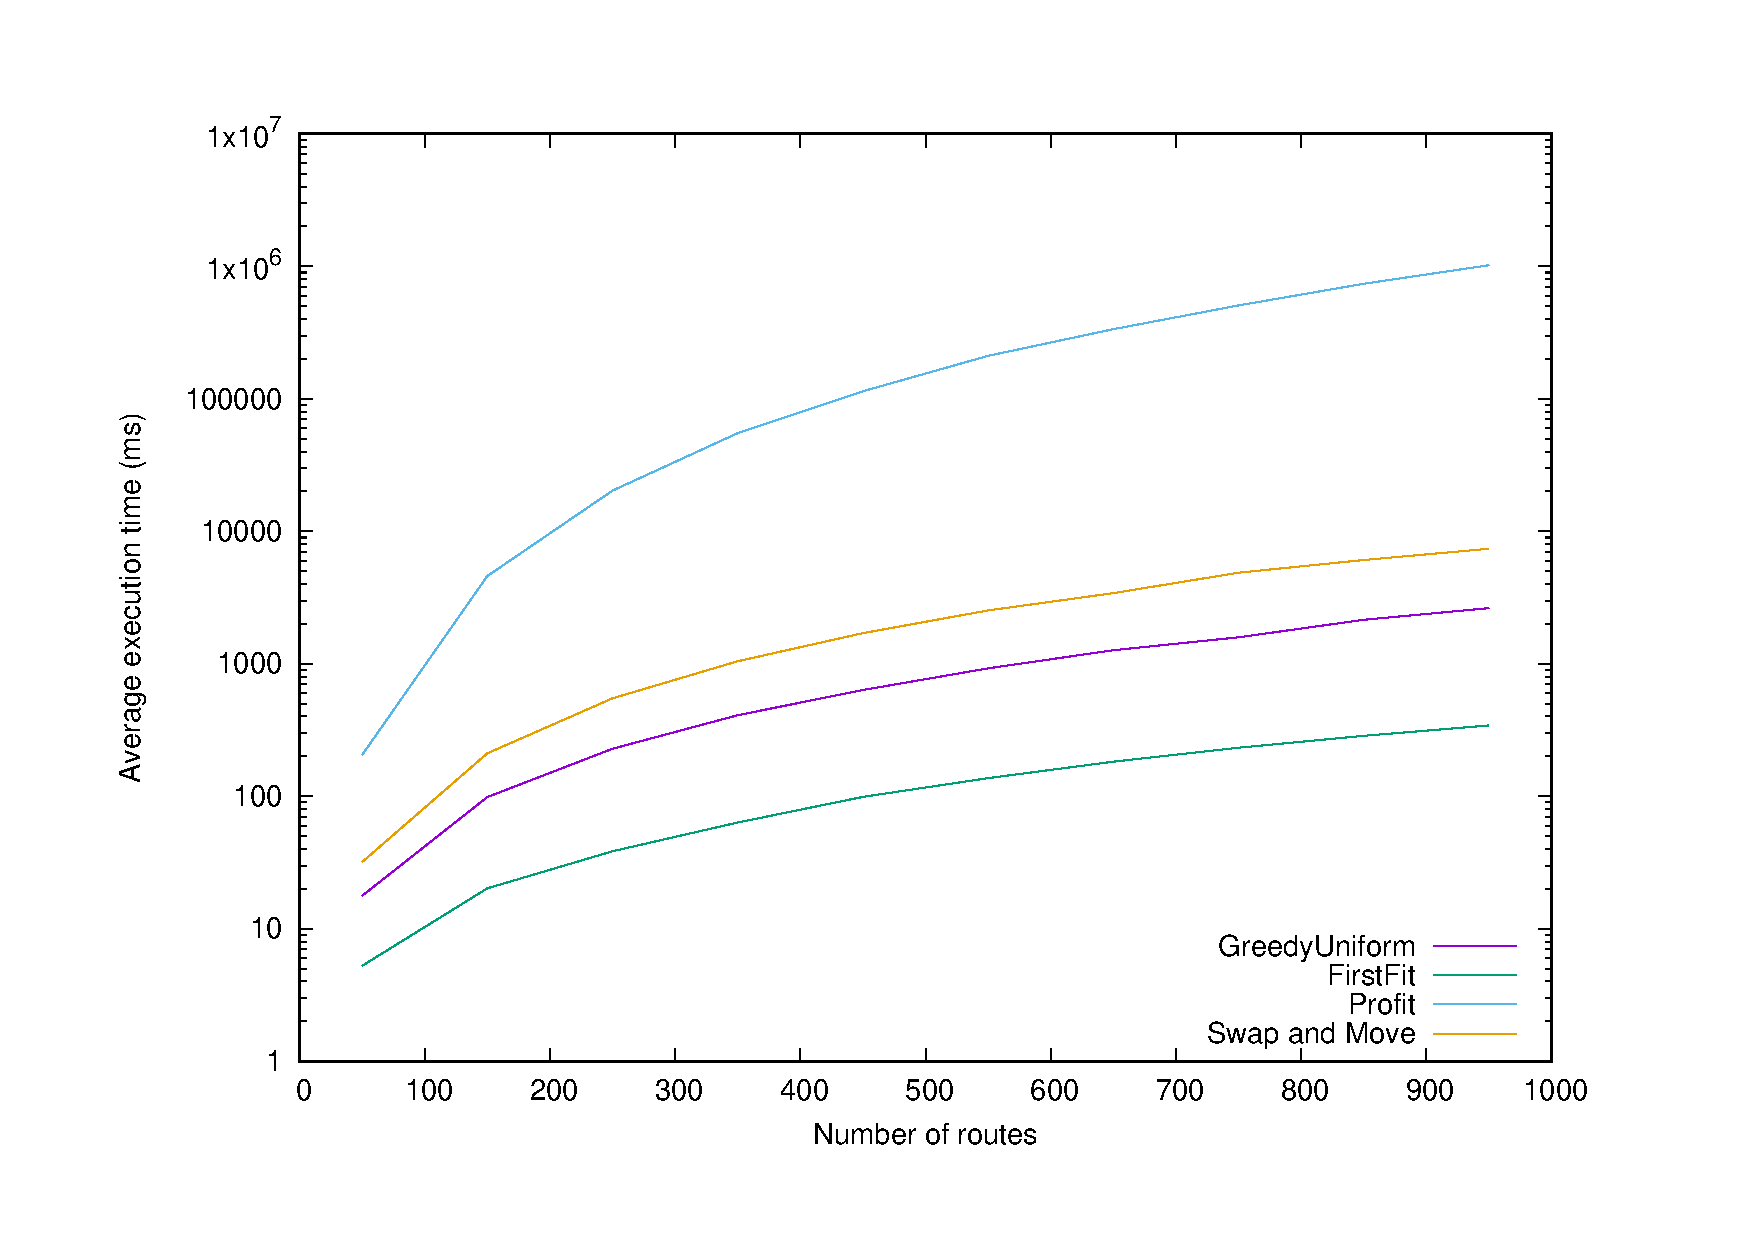
\includegraphics[scale=0.275]{Chapitre4PAZL/log}
\end{center}
\caption{Computation time (logarithmic scale) function of the number of datagrams of all algorithms on $10000$ instances of load $1$}
\label{fig:timelog}
\end{figure}


\section{From Large to Small Datagrams}\label{sec:reduction}

In this section, we explain how we can trade load or buffering in the network to reduce the size of datagrams down to $\tau = 1$. This further justifies the interest of Sec.~\ref{sec:small}, where specific algorithms for $\tau = 1$ are given.

\subsection{Datagram of Size One by Increasing the Load}

We describe here a reduction from an instance of \pma to another one with the same period and number of datagrams but 
the size of the datagrams is doubled. This instance is equivalent to an instance with $\tau = 1$, by dividing everything by the datagram size. Thus we can always assume that $\tau = 1$, if we are willing to double the load.


\begin{theorem}\label{th:double_load}
Let $I$ be an instance of \pma with $n$ datagrams and load $\lambda$. There is an instance $J$ with $n$ datagrams of size $1$
and load $2\lambda$ such that an assignment of $J$ can be transformed into an assignment of $I$ in polynomial time.
\end{theorem}
\begin{proof}
From $I = (P,\tau,(\notationdelay_{0},\dots,\notationdelay_{n-1}))$, we build $I' = (P, 2\tau, (\notationdelay_{0}',\dots,\notationdelay_{n-1}'))$, where $\notationdelay_i' = \notationdelay_{i} - (\notationdelay_{i} \mod 2\tau)$. The instance $I'$ has a load twice as large as $I$.
On the other hand, all its delays are multiples of $2\tau$ hence solving \pma on $I'$ is equivalent to solving it on $I'' = (P/2\tau, 1,(\notationdelay_{0}/ 2\tau,\dots,\notationdelay_{n-1} /2\tau))$, as already explained in the proof of Lemma~\ref{lemma:multiple}. 

Let us prove that an assignment $A'$ of $I'$ can be transformed into an assignment $A$ of $I$. 
Consider the datagram $i$ with offset $A'(i)$, it uses all times between $A'(i)$ and $A'(i) + 2\tau -1$ in the first period and all times between $A'(i) + \notationdelay_{i} - (\notationdelay_{i} \mod 2\tau)$ to $A'(i) + 2\tau -1+ \notationdelay_{i} - (\notationdelay_{i} \mod 2\tau)$ in the second period. 
If $\notationdelay_{i} \mod 2\tau < \tau $, we set $A(i) = A'(i)$, and the datagram $i$ of $I$ is scheduled ``inside'' the 
datagram $i$ of $I'$, see Fig.~\ref{fig:transf_2tau}. If $\tau \leq \notationdelay_{i} \mod 2\tau < 2\tau$, then we set 
$A(i) = A'(i) - \tau$. There is no collision in the assignment $A$, since all datagrams in the second period use
times which are used by the same datagram in $A'$. In the first period, the datagrams scheduled by $A$ use either the first
half of the same datagram in $A'$ or the position $\tau$ before, which is either free in $A'$ or the second half of the times used by another datagram in $A'$ and thus not used in $A$. 
\end{proof}
\begin{figure}[h]
\begin{center}

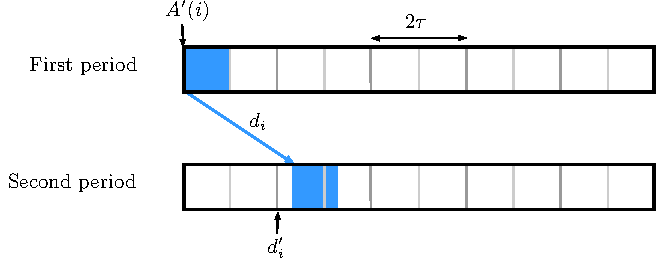
\includegraphics[scale=0.7]{Chapitre4PAZL/transfo2tau}
\end{center}
\caption{Building $I$ from $I'$ as explained explained in Th.~\ref{th:double_load}}
\label{fig:transf_2tau}
\end{figure}

Remark that combining Greedy Random and Theorem~\ref{th:double_load} allows to solve $\pma$ on random instances,
with probability one when the number of routes goes to infinity and the load is strictly less than $1/2$. 
This explains why we have not presented nor analyzed in details an algorithm designed for arbitrary $\tau$ on random instances, since any greedy algorithm, relying on optimizing $Fo(A)$, cannot guarantee anything for load larger than $1/2$.
However, in Sec.~\ref{sec:compacttuple}, we presented \compactfit, a simple greedy algorithm which exhibits good performance on random instances.

\subsection{Trade-off between Latency and Datagram Size}

The problem \pma is a simplified version of \pall, the practical problem we address, allowing a single degree of freedom for each datagram: its offset. We may relax it slightly to be more similar to what is studied in Chapter~\ref{chap:PALL}: we allow buffering a datagram $i$ during a time $b$ between the two contention points, which translates here into changing $\notationdelay_i$ to $\notationdelay_i + b$. The quality of the solutions obtained for such a modified instance of \pma are worst since the buffering adds latency to the datagrams. We now describe how we can make a trade-off between the added latency and the size of the datagrams, knowing that having smaller datagrams helps to schedule instances with higher load.


The idea is to buffer all datagrams so that their $\notationdelay_i$ have the same
remainder modulo $\tau$. It costs at most $\tau - 1$ of buffering, which is not
so good, since algorithms optimizing the latency do better on random instances, see~\cite{DBLP:journals/corr/abs-1801-07029}. However, it is much better than buffering for a time $P$, the only value for which we are guaranteed to find an assignment, whatever the instance. When all delays are changed so that $\notationdelay_i$ is a multiple of $\tau$, we have an easy reduction to the case of $\tau = 1$, by dividing all values by $\tau$, as explained in the proof of Lemma~\ref{lemma:multiple}.


We can do the same kind of transformation by buffering all datagrams, so that $\notationdelay_i$ is a multiple of $\tau / k$. The cost in terms of latency is then at most $\tau / k - 1$ but the reduction yields datagrams of size $k$.
For small size of datagrams, it is easy to get better algorithm for \pma, in particular for $\tau = 1$ as we have shown in Sec.~\ref{sec:small}. Here we show how to adapt \compactpair to the case of $\tau = 2$, to get an algorithm working with higher load.


\begin{theorem}
\compactpair on instances with $\tau =2$ always solves \pma positively on instances of load less than $4/9$.
\end{theorem}
\begin{proof}
We assume w.l.o.g that there are less datagram with even $\notationdelay_i$ than odd $\notationdelay_i$.
We schedule compact pairs of datagrams with even $\notationdelay_i$, then we schedule single datagram with odd $\notationdelay_i$. The worst case is when there is the same number of the two types of datagrams. In the first phase, if we schedule
 $n/2$ datagrams, the number of forbidden offsets is $(2 + 3/2)n/2 = 7n/4$. In the second phase,
 if we schedule $n/2$ additional offsets, the number of forbidden offsets is bounded by 
$ (1 + 3/2) n/2  + (1 + 1)n/2 = 9n/4$. 
Hence, both conditions are satisfied and we can always schedule datagrams when $n \leq (4/9)m$.
\end{proof}

We may want to add less latency to the datagram using the longest route. A natural idea is to choose the datagram with the longest route as the reference remainder by subtracting its remainder to every delay.
As a consequence, this datagram needs zero buffering. However, the datagram with the second longest route may have a remainder of $\tau -1$, thus the worst case increase of total latency is $\tau -1$. 

Another aim would be to minimize the average latency rather than the worst latency.
We prove that we can do the transformation yielding $\tau=1$ while optimizing the average latency. 
 The only degree of freedom in the presented reduction is the choice of the reference remainder since all other delays are then modified to have the same remainder. Let us define the total latency for a choice $t$ of reference time, denoted by $L(t)$, as the sum of buffering times used for the datagrams, when $t$ has been removed from their delay.
If we sum $L(t)$, from $t=0$ to $\tau-1$, the contribution of each datagram is $\sum_{i=0}^{\tau-1} i$. Since there are $n$ datagrams, the sum of $L(t)$ for all $t$ is $n \tau (\tau-1)/2$. There is at least one term of the sum less than its average,
hence there is a $t_0$ such that $L(t_0) \leq n (\tau-1)/2$. Hence, the average delay for a datagram, with $t_0$ as reference is less than $(\tau -1)/2$.


\section*{Conclusion}
  \addcontentsline{toc}{section}{Conclusion}
In this chapter, we study the problem \pazl that is finding periodic assignments without buffering on star routed networks, a routed network with two serial contention points.  
We show that for messages of arbitrary size, there is always a solution as soon as the load of the network is less than $40\%$.
To do so, we propose several greedy algorithms of increasing sophistication. They rely on optimizing different measures of how many positions there are in the second period,
given a partial assignment and any new datagram to schedule. 
We give a canonical representation of an assignment, whose compactness allow to derive an FPT algorithm to solve \pma parametrized by the number of routes. When the number of routes is less than $20$, we can thus find in reasonable time an optimal solution to \pma. 


For messages of size $1$, we prove that it is always possible to schedule them, when the load is less than $61\%$ using a polynomial time algorithm.
The algorithm relies on optimizing a potential, which represents, given a partial assignment, how many possible positions there are for the datagrams not yet scheduled. 
The algorithm is not greedy, contrarily to those presented for the case $\tau > 1$, since optimizing the potential requires a procedure of local optimization 
which exchange a scheduled datagram with an unscheduled one.  
Furthermore, we study the simplest random greedy algorithm solving \pazl, and show that, for a given load lower than one, almost all instances admit a solution with high probability, explaining why most greedy algorithms work so well in practice.  
The study of the special case of $\tau = 1$ is then justified, by providing several reductions from $\tau >1$ to $\tau =1$,
while increasing the load or the latency only mildly.


The performance of the presented algorithms over average instances are shown to be excellent empirically (\compactfit for large $\tau$ and \swapandmove for $\tau = 1$) for loads up to $0.7$, for tens to hundreds of datagrams. Hence, we can use the simple algorithms presented here to schedule C-RAN datagrams \emph{without using buffer nor additional latency} in polynomial time, if we are willing to use only half the bandwidth of the shared link.

Several questions on \pma are still unresolved, in particular its $\NP$-hardness
and the problem of doing better than load $0.5$ for arbitrary $\tau$ and random instances.
We could also consider more complex network topologies with several shared links, most presented algorithms (\firstfit, \metaoffset, \compactpair, \swapandmove)
could easily be adapted to this context.
On star routed network, our experiments show that most of the time, there is a solution for \pma when the load is under $0.8$, but not for higher loads. Hence, in the next chapter, we study the problem \pall on highly loaded star routed networks. Problem \pall gives an higher degree of liberty to build assignments by allowing a buffer in one contention point of the network, at the cost of some additional latency. 